\chapter{Capacitive Load Cells for Underground Mining Force Sensing Applications
\label{chap:P3}}

\begin{center}
This article has been published open access and is part of the public domain.
The copyright remains property of the author.
\end{center}

\subsection{Abstract}

Cutting force is strongly correlated to both tool wear and material type.
In underground coal mining, machine operators put themselves at risk when 
getting close to the machine or cutting face to observe the process.
Long term exposure to these conditions also inevitably leads to health issues.
To improve safety and efficiency of machine operators, 
we propose a cutting force sensor.
The sensor design is tested using a linear cutting machine with two separate coal samples
cast in concrete cut with conical pick cutters. 
We use cutting penetrations of 1.0 and 1.5 inches and vary tool wear using picks with artificially worn
spherical tips to test a range of conditions.
Measurements from both the custom sensor and sensors embedded in the test equipment are collected.
Using 100 random splits of the collected data, we fit linear and neural network regression models
with 30\% of the data for training and the rest for testing. 
The normal force exceeds 60 kN during our rock cutting tests,
and it is averaged using a low pass filter with a 10 Hertz cutoff frequency.
The sensor is able to track the normal force on the conical picks with a 
mean absolute error less than 6 kilonewtons and an $R^2$ score greater than 0.60 using a linear regression.
The use of a small neural network and a 2nd order polynomial expansion is able to 
improve this to a mean absolute error less than 4 kilonewtons and an $R^2$ score around 0.80 when the 
sensor measurements are also filtered with a low pass filter before the regression.
This type of sensor could allow operators to assess tool wear and material type
using objective force measurements while maintaining a greater distance from the cutting interface.

\subsection{Introduction}\label{sec1}

The health and safety of underground coal miners is affected by 
nearly every aspect of the operation \cite{Khanzode2011}.
The effects of these hazards are mitigated by proper ventilation and extraction planning \cite{Saleh2011}.
Machine operators need feedback from the cutting interface to achieve the planned extraction \cite{Bartels2009},
but the cutting interface is the source of harmful dust, gasses, and tunnel conditions.
Our proposed sensor can collect force data from individual conical picks at the cutting interface, 
providing operators more feedback while allowing them to maintain a greater distance.

In the U.S.A., employment in the coal mining sector has generally 
decreased since the 1970s boom, but experienced a brief renaissance during 2000-2010 \cite{Betz2015}.
Employment in coal mining in the U.S.A roughly halved over the period between 2010 to 2020 \cite{FRED2023}.
Allocation of resources that reduce accidents and increase mine output is 
the optimal trajectory for advancing technology in underground coal mining \cite{Sider1983}.
If worker supply continues to decline and regulations increase,
boosted worker productivity will be needed to meet future demand for coal.

Coal is generally a soft rock and can be broken apart by the average set of human hands in small quantities.
The rock in which coal is often deposited is much harder, 
and is cut by a continuous mining machine with a drum holding an array of conical picks.
Specific energy of the cutting process has a strong correlation with material type and tool wear \cite{TEALE196557}.
We choose to design a sensor that measures the forces present on the picks. 
These force measurements provide direct and objective feedback from the cutting process.

This work is the follow-up research for our previous sensor design, 
which used a much thinner membrane, 25 $\mu$m thick, with non-linear deformation dynamics,
between two electrodes \cite{oltmanns2023low}.
Here, we test a design with a much thicker dielectric, 
with nominal thickness of 240 $\mu$m, and a single conductive plate.
In this work, we also propose a network topology for efficient use of the sensor
in the underground mine. 
The force sensor fits under the sleeve of a conical picks, 
and can provide real time force feedback from the location of the tool.
Operators must make decisions regarding tool changes and cutting strategies.
This device would assist operators by providing measurements of the rock cutting forces
present at each instrumented pick, allowing them to make decisions from more remote locations.

Such a device would also be able to log measurements for later analysis and process optimization.
The design and validation of a single smart bit sensor is the focus of this article.
In \ref{fig:network_proposal}, we propose a larger network that integrates the sensor
and illustrates end applications.
The sensor measurements would be collected and forwarded to operators wirelessly 
so they can make decisions with more information.
Additional description of the proposed network is given in the Background subsection.

\begin{figure}[t]
\centering
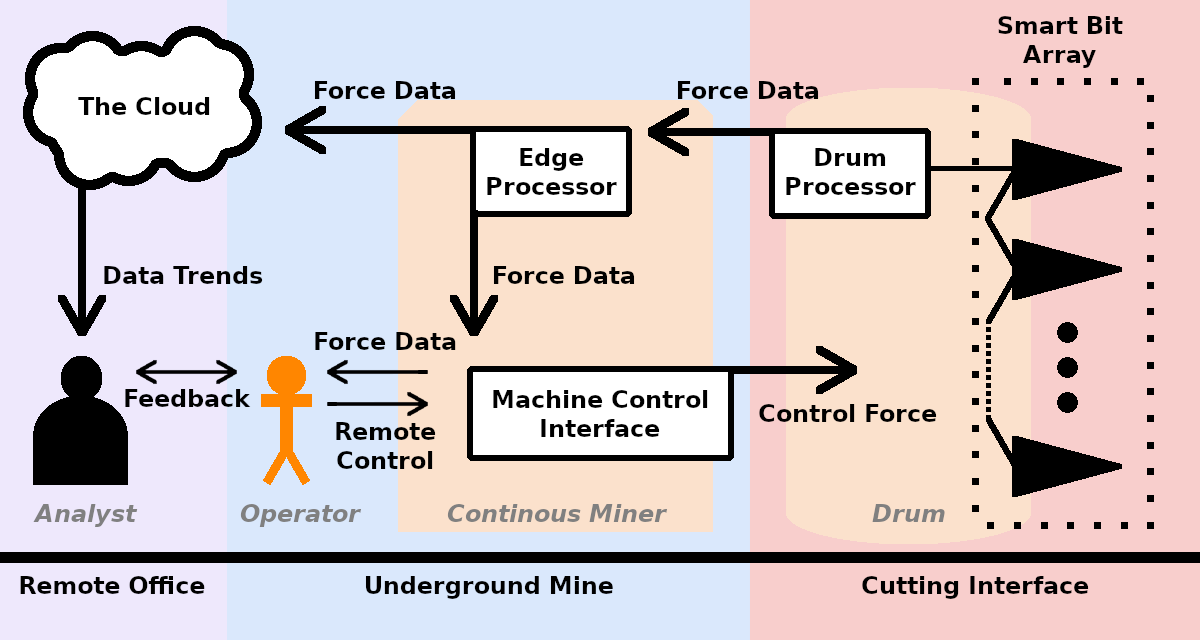
\includegraphics[width=4.5in]{p3_media/figures/dataflow.png}
\caption{The network proposed for integrating our sensor with the continuous miner.
Individual sensors can be linked to an edge processor on the drum which aggregates the force data via CAN bus,
a robust interface for sensor networks. From the edge processor on the drum, labeled "Drum Processor",
force data can be sent wirelessly to an edge processor on the machine chassis. 
There, the data can be parsed into a displayable format for
immediate use by the machine operator and also sent up to the surface to be stored in a central server for 
processing by a mine analyst to gain insight into operator performance. 
The analyst and the operator can then communicate to increase efficiency and safety.}
\label{fig:network_proposal}
\end{figure}


The rest of this article is organized as follows:
The Background subsection covers how our sensor could be integrated with the mine and
general motivation and principles for using capacitive sensors.
Following the Background subsection is the Methods subsection, 
which discusses our experimental setup, 
the regression techniques used for the empirical models,
and the analytical modeling for our sensors. 
Then, the Results subsection shows data from the calibration and test procedures, 
sharing empirical values for sensitivity 
and comparisons of force predictions using the sensor measurements 
with measurements from the test equipment.
Finally, a Discussion subsection mentions both benefits and drawback to our implementation
while the Conclusion subsection shares potential impacts from this technology.

 
\subsection{Background}

In order to integrate our sensor with the mining workflow, we propose the network topology 
shown in \ref{fig:network_proposal}. This figure shows multiple smart picks 
connected via CAN bus, which has been recognized as meeting the requirements for 
other underground coal mining applications \cite{Shu2010, Ma2021}. 
The data from the smart picks is aggregated and compressed by an edge processor on the drum,
which we refer to as the drum processor.
From the drum processor, data is both sent wirelessly to the 
operator in real time and to a central storage server, a.k.a. the cloud. 
The information could be displayed to the operator using a backlit display 
on the remote controls for the machine.
The data in the cloud can be analyzed to identify trends in production efficiency and safety. 

Instrumenting each pick, or a representative subset, allows capture of cutter-head state,
which is necessary for operators to make informed decisions 
regarding tool change scheduling and machine control. 
This setup also allows the human operator to make informed decisions using the collected feedback
while staying in a safer position. 
This could aid in identifying if the tool force is much greater than expected,
reducing incidences of operators approaching the machine to check tool wear.

This work focuses on the design of the force sensor at the cutting interface.
When it comes to designing a force sensor for underground mining applications, 
several base designs and materials were considered. 
In general, rock cutting forces depend on the tool geometry and the material properties and
they can range from dozens to hundreds of kN at each pick \cite{Zeng2021, Fan2023, Roxborough1981, Bilgin2006}
The operation of the mining equipment and the complicated network of jagged tunnels cause the 
environment to be noisy electromagnetically and acoustically
\cite{Ikeda2021, Seguel2022, Yarkan2009, Thrybom2015, Ranjan2014}. 
The mining environment is also very harsh, and cutting tools can be consumed quickly, 
typically being consumed after clearing several cubic meters \cite{Hurt1985, Su2020, Rostami2003}.
These conditions require any sensor to be robust and also low cost.

It has long been known in rock cutting that the specific energy of a material being removed 
is related to its strength when breaking down \cite{TEALE196557}.
Also, when a conical pick wears down to a rounded shape, the specific energy of the cutting process
increases, resulting in less cutting efficiency and higher forces \cite{Zeng2021}.
In an underground coal mine, operators directly use many cues 
from the environment to determine tool wear levels and material types \cite{Bartels2009}.
Objective feedback in the form of force measurements stands to improve operator efficiency.

Other methods, like vibro-acoustic signal processing, 
are gaining popularity for tool wear and material classification 
in domains like metal milling \cite{Cooper2020} and oil drilling \cite{Wang2023}.
Acoustic techniques can be susceptible to interference from nearby sources, 
but a force sensor on the pick will have a direct link to the cutting process.
Many different technologies exist for detecting 
roof fall conditions \cite{en15218312, SLAKER201783, alzahrani2017detection}.
Our technology would help mitigate unintentional roof damage by directly measuring
cutting tool force and facilitating either operators or machine safety features
to rapidly respond.

To measure forces in a tough environment with a low cost sensor, 
we design a capacitive sensor enclosed in a steel case with a polyimide dielectric. 
We use the simple parallel plate approximation for our capacitive sensor:
\begin{equation}
\label{eq1}
C = \frac{\epsilon A}{d},
\end{equation}
where $C$ is the resulting capacitance, $\epsilon$ is the absolute permittivity of the dielectric, 
$A$ is the area of overlap between the plates, and $d$ is the distance between them \cite{HyperPhysics}. 
Fringing effects are small compared to the nominal capacitance at the resting displacement \cite{Reichert2020}.
The sensor is designed so force compresses the sensor, altering the $d$ value in (\ref{eq1}) \cite{Dobrzynska2012, Zhu2020}. 
Other sensor designs involve co-planer electrodes \cite{Lu2016, Zaitsev2017, Barile2019}, different dielectrics \cite{Nelu2019},
or motion parallel to the plates \cite{Kim2005, Liu2016, Prit2019}.
We design our sensor to be compressed normal to the plates for a robust design that 
can withstand the forces of rock cutting.

\subsection{Methods}

For our design, we first choose the required 
force sensing range, bandwidth, accuracy and resolution.
A force sensing range of 0 to 200 kN is targeted.
For bandwidth, we are interested in tracking average,
 rather than instantaneous, cutting force because tool wear and material type 
are known to change average cutting forces.
Tracking high frequency changes in cutting force can be useful 
for classification of material type and tool wear, as shown in our previous work \cite{oltmanns2023low}.
Using lower frequencies for regression de-emphasizes the 
differences in dynamics between our sensor and the test equipment sensors
caused by their distance and individual designs by focusing on the average forces.

The regression target is chosen to be the drag force after it is filtered 
with a low pass filter with a 10 Hz cutoff frequency.
Making the regression target an average lowers the variance that must be estimated.
This relaxes the regression problem, but still gives a sensor with known accuracy and response time.
The requirements for accuracy and resolution are not very stringent due to the large differences 
in forces that can be expected between distinct materials and wear conditions.
In terms of mean absolute error, 15 kN or less would enable basic
classification of material and wear conditions.

%The limiting factor for system bandwidth in the underground mining scenario is the resonant 
%frequncy of the cutting implement, which is much less stiff than the rock face when cutting hard rocks.
%To avoid aliasing, the sensor should be more stiff than the mining machine
% but also must be of similar stiffness to the rock cutting tool or else the sensor will not detect the cutting forces. 
%Regarding accuracy, the sensor must be able to reliably detect changes in average cutting forces
%with minimal drift or bias and a known sensitivity.

\begin{figure}[t]
\centering
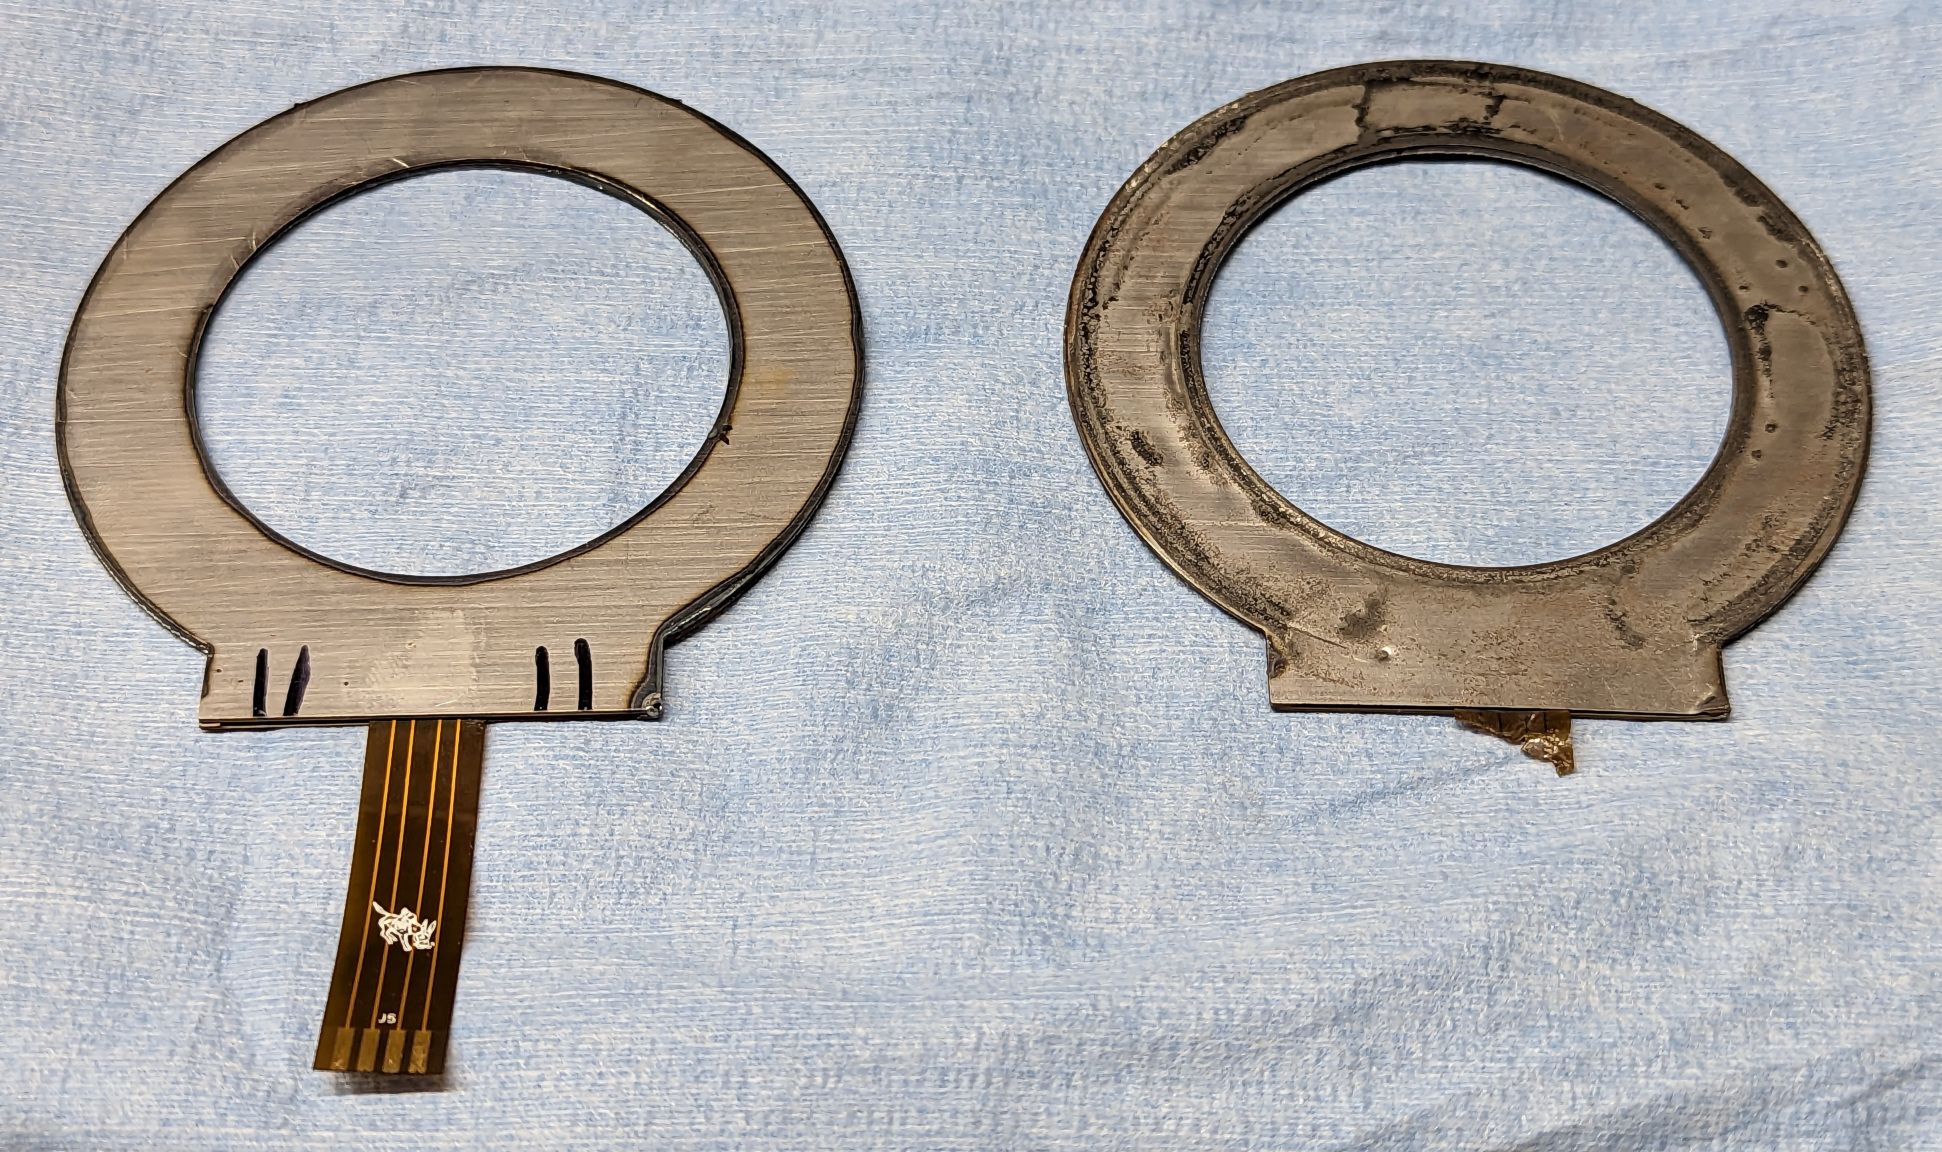
\includegraphics[width=4.5in]{p3_media/figures/sensors_intact_crushed_cropped.jpg}
\caption{Two sensor prototypes. The one on the left has only been used for characterization 
in a load cell with controlled parameters. The one on the right has been through the same 
calibration as well as a controlled rock cutting experiment. During the rock cutting experiment,
the air gap of the sensor is crushed out, altering the model but still giving a mostly linear sensor.
The exposed sensor membrane was inadvertently cut by the edge of the second sample on the last cut.
The walls of the sensor have retained much of their thickness, but they have deformed slightly to 
match the tooling.}
\label{fig:sensors_prototypes}
\end{figure}

Finished samples of our sensor design are shown
in \ref{fig:sensors_prototypes}.
We conduct two types of experiments with our sensor, load frame testing and rock cut testing.
Both tests use the FDC2114 from Texas Instruments to record the 
capacitive data from each of the 4 channels at roughly 400Hz. 
The load frame test measures the sensor response to gentle load profiles in a controlled environment
and the rock cut testing demonstrates use of the sensor for the application.

For the load frame testing, we apply load profiles which ramp up to 200 kN 
then back down at rates of 2, 4, 6, 8 and 10 kN/s. 
We examine the relationship between the sensor measurements 
and the force and strain measurements from the load frame.
With this test, we can measure the sensor linearity and characterize the noise
in a controlled environment. 
We also measure the sensitivity to normal force with a linear regression.
One of the samples is tested twice to characterize repeatability.
The setup is shown in \ref{fig:loadframe}.


\begin{figure}[t]
\centering
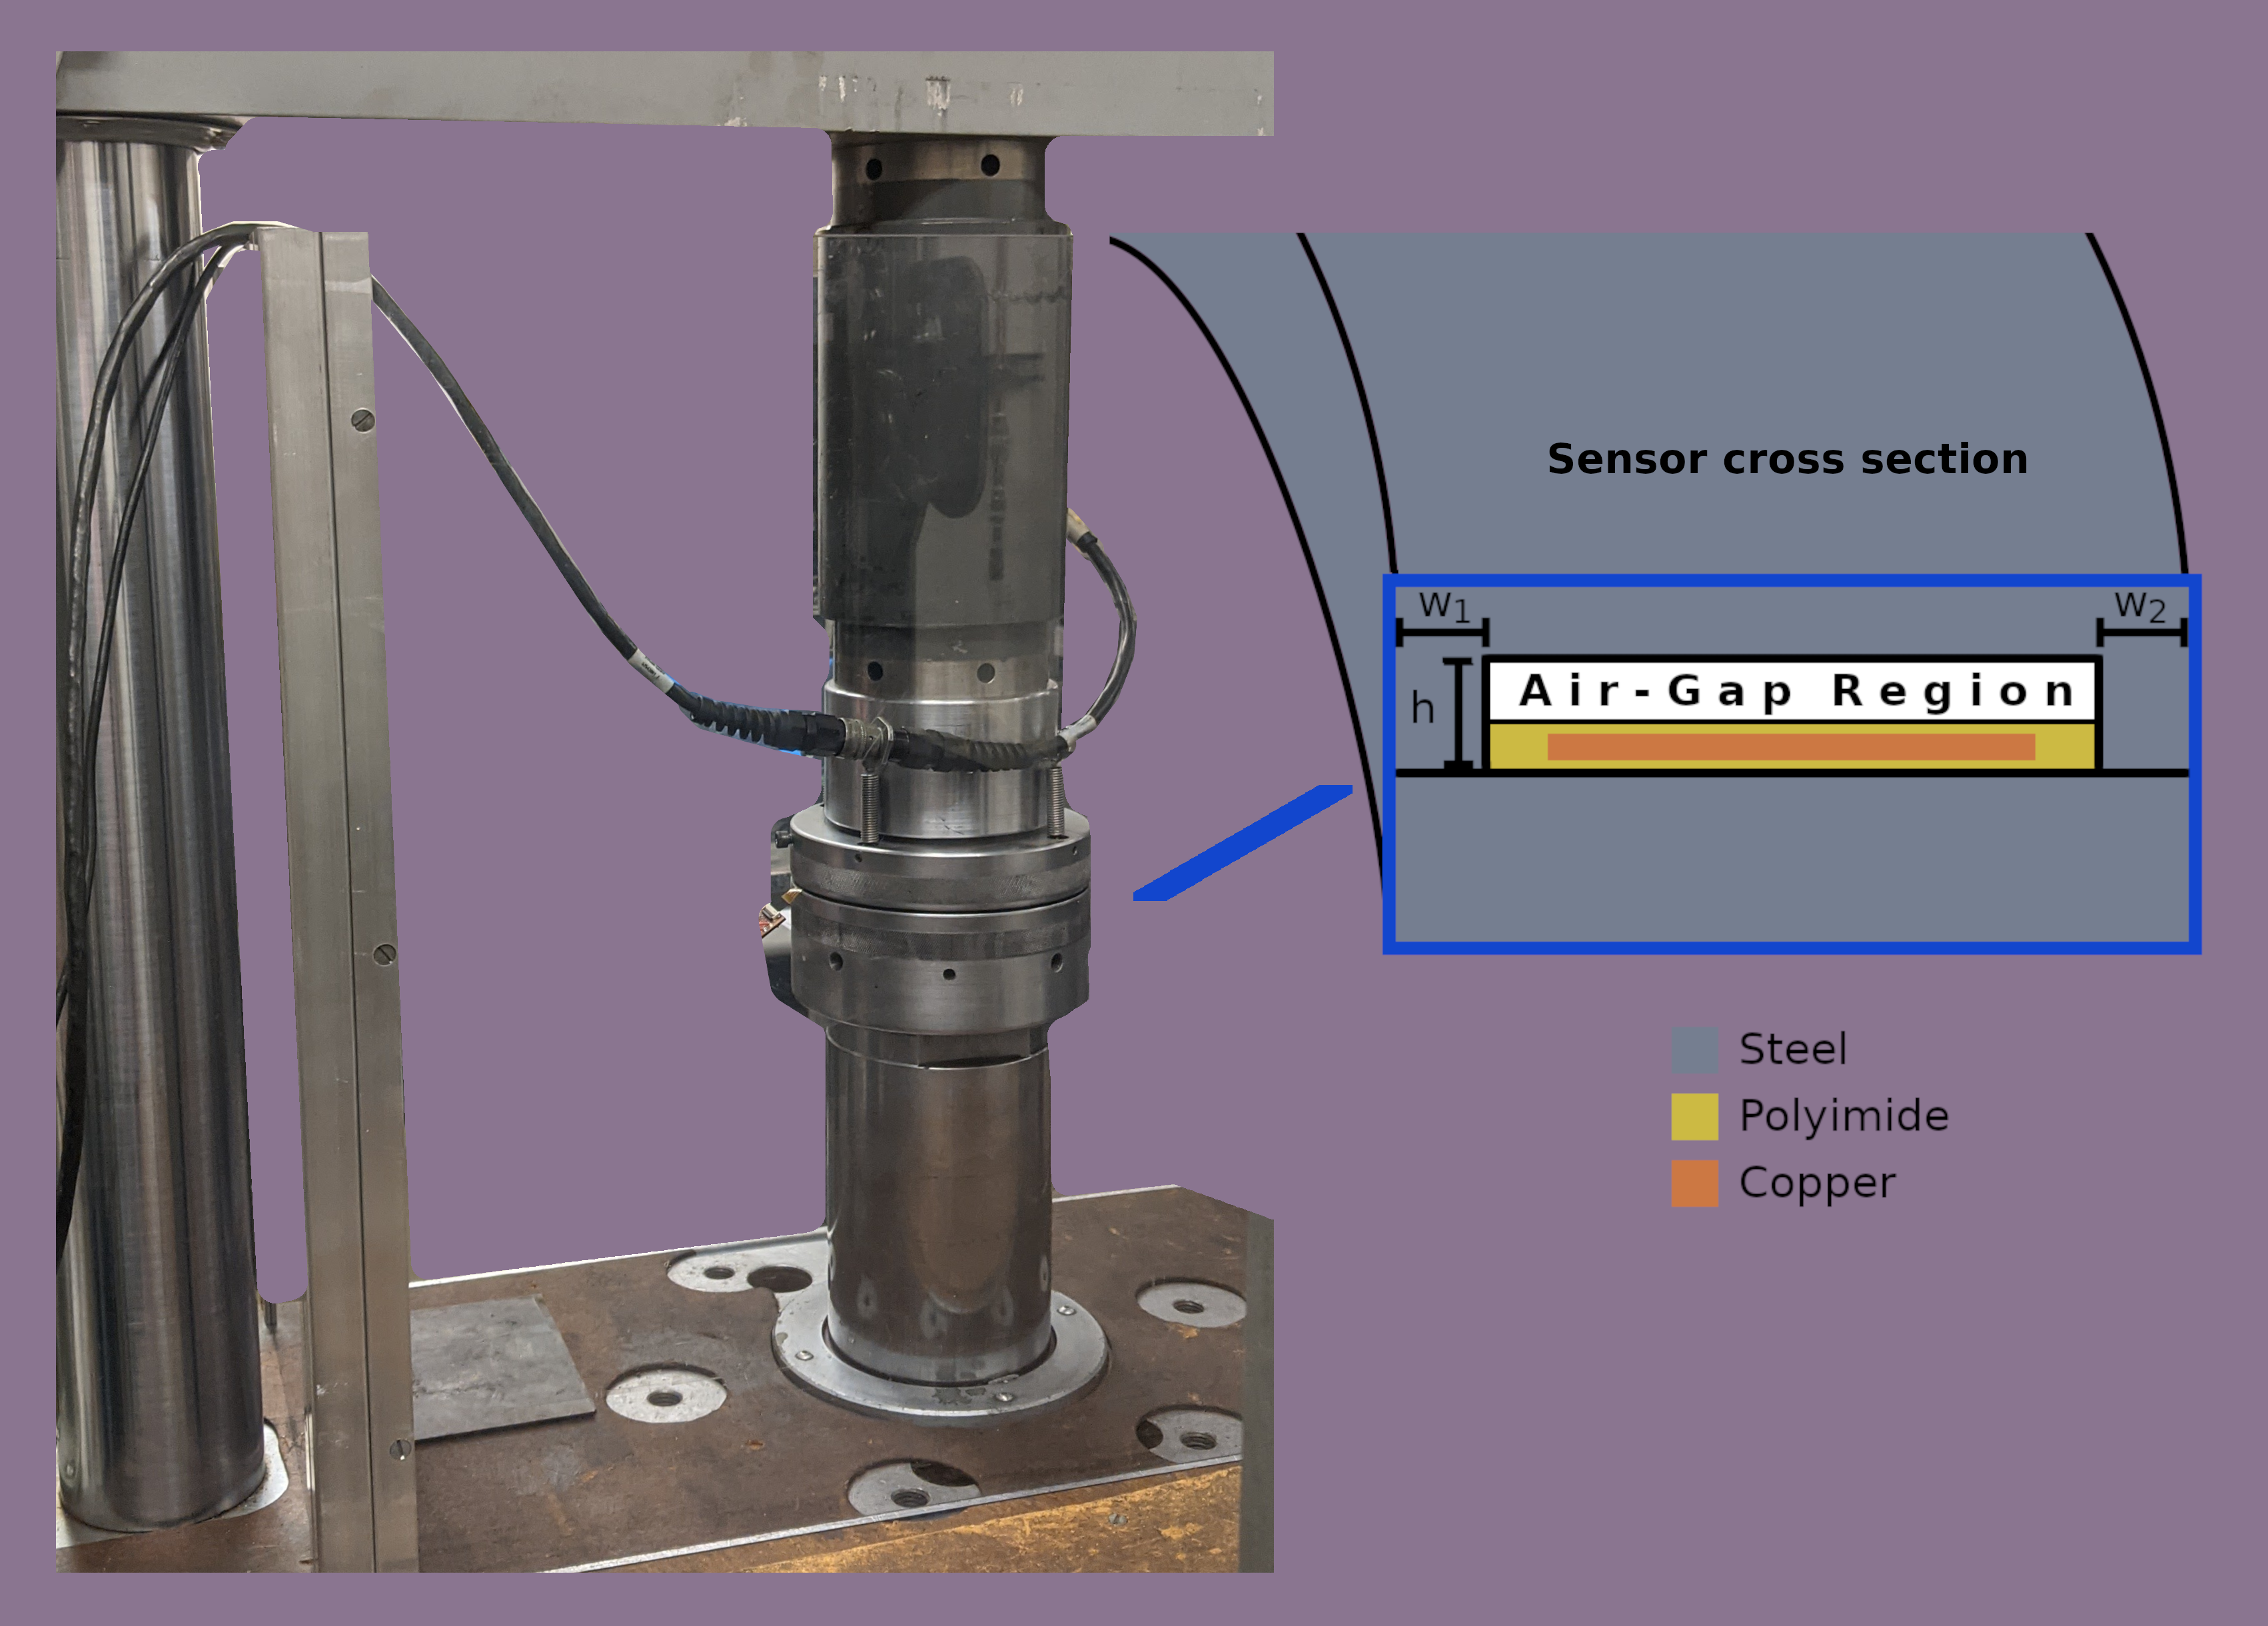
\includegraphics[width=4.5in]{p3_media/figures/load_frame_highlight.png}
\caption{The setup for the load frame characterization of the sensor in the air-gap configuration, 
shown in the sensor cross subsection.
The load frame applies a controlled loading profile to the sensor, allowing the response of the sensor
to be compared against a controlled input. The load frame measures both force and displacement while
the sensor's capacitance is measured by the interface circuit.
Forces in this test ramp up to 200 kN and back down at a controlled linear rate.}
\label{fig:loadframe}
\end{figure}

For the rock cut testing, we use the linear cutting machine at Colorado School of Mines
Earth Mechanics Institute, shown in \ref{fig:lcm}. 
Two samples of coal embedded in concrete were cut 
using conical picks instrumented with one of the sensors.
Wear and depth of cut are varied for the tests.
The conditions for the test and the number of samples for each condition are shown in \ref{tab:data}.
The cutting speed was 25.4 cm/s (10 in./s).
%The conical picks were varied in wear from new condition to worn condition with a moderately worn condition in between.
%The depth of penetrations tested were 1.0 and 1.5 inches.
In this test, the sensor changes to the crushed gap configuration,
and we can fit empirical models to transform the sensor measurements into 
normal force on the tool.

\begin{table}[]
\centering
\caption{Rock cut conditions tested, coal samples and conical picks}
\label{tab:data}
\begin{tabular}{|l|l|l|}
\hline
Depth of Cut             & Wear Condition (Tip Diameter) & Number of Cuts \\ \hline
1.0 in.                  & New (3.71 mm)  & 10             \\ \hline
1.5 in.                  & New (3.71 mm)  & 2              \\ \hline
1.5 in.                  & Mod (17.9 mm)  & 4              \\ \hline
1.5 in.                  & Worn (27.5 mm) & 5              \\ \hline
 & Total & 21 \\ \hline
\end{tabular}
\end{table}

\begin{figure}[t]
\centering
\includegraphics[width=5.0in]{p3_media/figures/rock_cutting_setup_detail.png}
\caption{The setup for the rock cutting experiment. Strain gauges measure the forces on the cutting tool from
close proximity while hydraulic actuators drag the rock sample against the cutting tool. The sensor is 
located between the sleeve and the block of the cutting tool, as shown in the profile view diagram.
In this setting, the sensor is in the crushed gap configuration, shown in the sensor cross subsection.
Forces in this test are less than 100 kN, but the rate of change of force is large and variable.}
\label{fig:lcm}
\end{figure}


For this study, we used different mathematical models to describe the 
two tests performed with the sensor.
For the load frame tests, the sensor sensitivity is low, but demonstrates
the working principle of the sensor in a controlled environment.
For the rock cutting tests, the sensor sensitivity is much greater.
This can be explained by plastic deformation compressing the sensor 
to a new configuration and our analytical models describe how this can increase sensitivity.

Due to the large number of design parameters,
 we leverage data-driven methods to formulate
the relationship between measurements and normal force on the tool.
Our models show that the system in nonlinear, so we use a 2nd order polynomial
expansion to allow the regression models to compensate more accurately.
The analytical models for both sensors are described in the following subsubsection.
After that, the next subsubsection discusses the regression techniques used 
to estimate cutting drag force from the sensor measurements.

\subsubsection{Analytical Modeling}
To model the relationship between input force and measured resonant frequency, 
we represent the sensor in isolation and allow for slight parasitic capacitance and inductance
when comparing the model to the experimental results. 
The FDC2114 Capacitance to Digital Converter
is used to measure the resonant frequency of all four sensor channels.
This setup has a resolution of 2.44 kHz per bit, and uses
a reference frequency of 40 MHz and an internal gain setting of 2.
With this configuration, the converter can measure resonant frequencies up to 4 MHz.

%The chosen capacitance to digital converter measures the resonant frequency of each channel of the load cell
%with a max sample rate of around 400 Hz for a 4 channel load cell.
%The thin walls of the sensor give it a high physical bandwidth and 
%the resonant frequency of our cutting equipment is known to be around 80 to 100 Hz,
%so we should expect to capture the dominant modes of the system as variations 
%in the sensors resonant frequency as measured by the converter.

%We calculate the nominal capacitance of an individual sensor element by applying the parallel plate model,
%given in Eq.~\ref{eq1}, 
%to each region of the sensor.
%The regions, denoted $r_{1}$ to $r_{3}$ for the air gap sensor and $r_1$ and $r_2$ for the crushed gap sensor, 
%the individual capacitance of the region is approximated by the parallel plate equation:
%\begin{equation}
%C_{r_n} = \frac{\epsilon_{r_n} A}{d_{r_n}},
%\end{equation}
%where $C_{r_n}$ is the capacitance in Farads for region number $n$, 
%$\epsilon_{r_n}$ is the absolute permittivity of the dielectric in the region, 
%$A$ is the area of the plate, 
%and $d_{r_n}$ is the thickness of the dielectric in the region.
%We the apply the series and parallel circuit equations for capacitors according to the model
%and determine the resonant frequency of the sensing circuit as a function of input force.

The resonant frequency of the sensing circuit is that of a parallel inductor and capacitor \cite{Nilsson2015}:
\begin{equation}
f = \frac{1}{2\pi\sqrt{L_b [C_b + C_s]}},
\end{equation}
where $L_b$ is the lumped inductance from the board and parasitic, 
$C_b$ is the lumped capacitance from the board and parasitics,
and $C_s$ is the capacitance for the sensor element, which is electrically parallel to $C_b$.
We use this model to explore the trade-offs in performance and 
changes in sensitivity between the two models.
To describe the different design aspects of the sensor performance, 
the chain of derivatives from resonant frequency to input force:
\begin{equation}
\frac{\partial f}{\partial F_{in}} = \frac{\partial f}{\partial C_s} \ \frac{\partial C_s}{\partial d_r} \ \frac{\partial d_r}{\partial F_{in}},
\end{equation}
is helpful. 
We explain the significance of each term on the right hand side below.

It was found during calibration and
testing that it is necessary to model both the air gap sensor, and a sensor with a crushed air gap.
The model with the air gap explains the characterization experiment with good accuracy, while the
model with the crushed air gap explains the rock cutting experiment with good accuracy. 
The crushing of the air gap suggests that rock cutting produces large forces on the cutting tools.
The character of the sensor deformation can be seen in \ref{fig:sensors_prototypes}
Model diagrams for both modes of sensor operation are shown in \ref{fig:sensors_models}.
The first term on the right hand side, the sensitivity of frequency to sensor capacitance 
is the same for both of our sensor configurations. The other two terms are unique to each model.

\begin{figure}[t]
\centering
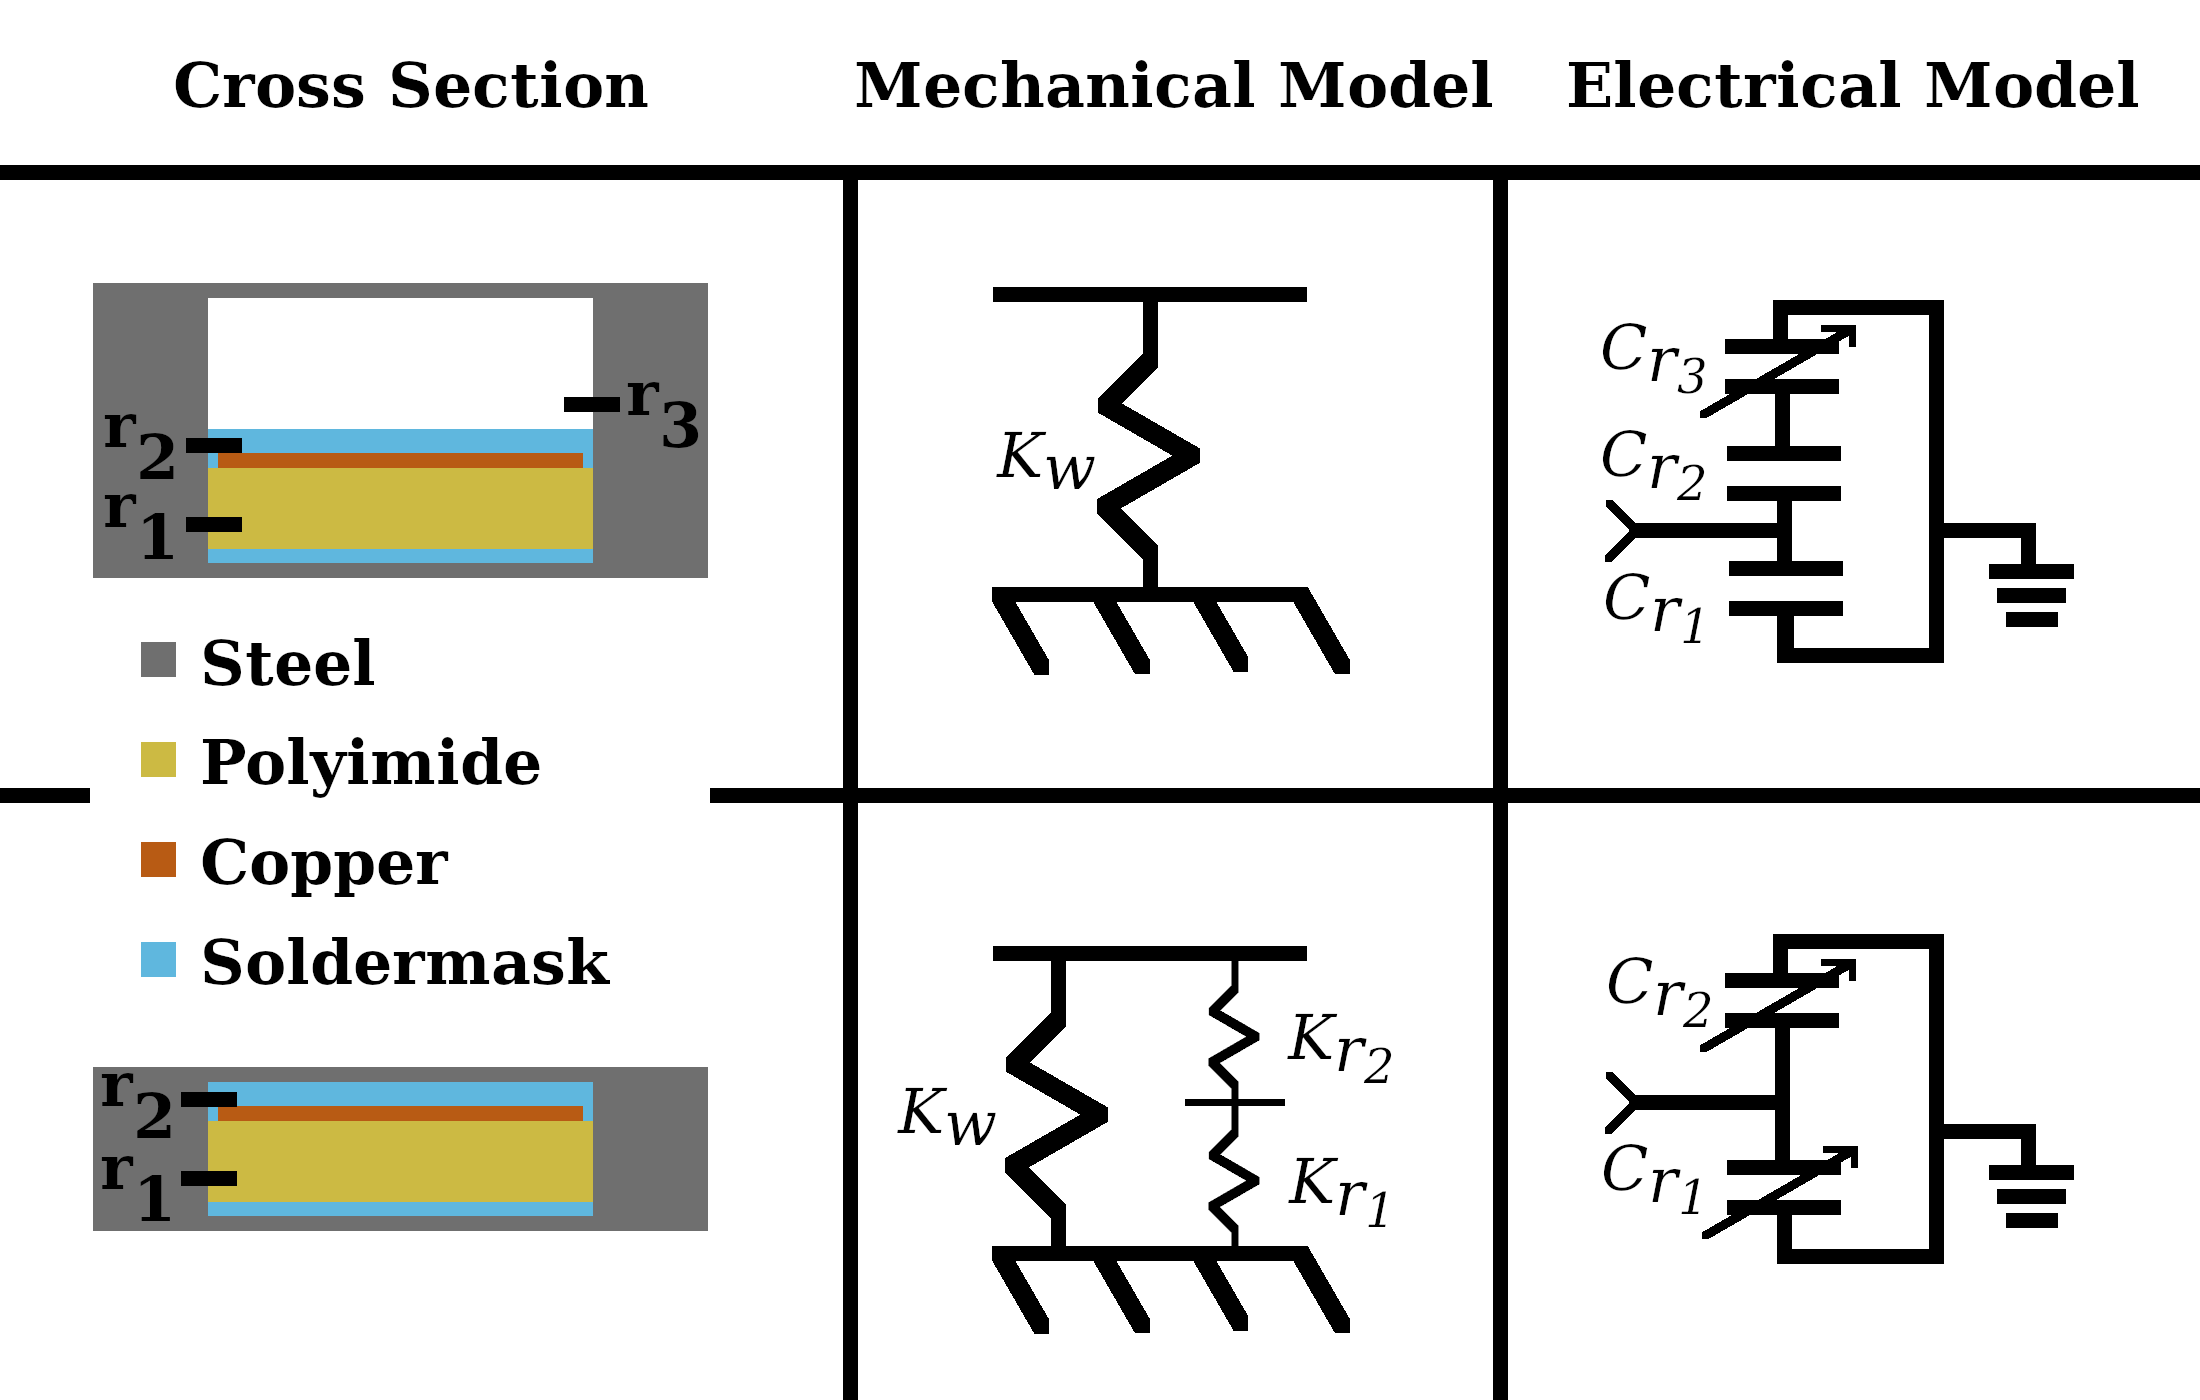
\includegraphics[width=4.5in]{p3_media/figures/model_fig2.png}
\caption{Cross subsection models for the two sensor modes. The top model has the air gap intact, 
resulting in one region which has variable capacitance. The bottom model has a crushed air gap, 
resulting in a stiffer sensor with two regions of variable capacitance. The top model is valid 
for sensors which have not undergone significant plastic deformation, while the bottom 
model is accurate for sensors after they have formed to the cutting tool.
The measured stiffness of the case in the air gap configuration, $K_w$, 
is around 780 meganewtons/meter. 
In the crushed gap configuration, the polyimide 
occupies more than twice as much area as the steel walls and is very thin in comparison.
We lump the soldermask and polyimide together for the model of $r_1$ since the soldermask is
thin in comparison to the polyimide and has similar properties. 
}
\label{fig:sensors_models}
\end{figure}

The sensitivity of sensor frequency with respect to sensor capacitance is:
\begin{equation}
\frac{\partial f}{\partial C_s} = \frac {-L_b}{4 \pi \bigg(L_b(C_b + C_s)\bigg)^{\frac{3}{2}}}.
\end{equation}
If all other parameters are held constant, 
larger $C_s$ values will give less sensitive sensors. 
The second derivative has a similar shape, indicating that while less sensitive, 
larger $C_s$ values will have more linear responses. To understand how the sensor
responds to strain, the next term, the sensitivity of capacitance to displacement, is needed.

For the air gap sensor, $r_3$ is the region where thickness varies with the input force.
When considering the crushed gap sensor, both $r_1$ and $r_2$ will deform, with most of the
deformation happening in $r_1$ since it is less stiff in comparison to the much thinner $r_2$. 
The air gap sensor is less stiff than the crushed gap sensor, as the polyimide is 
much stiffer than the thin steel walls of the sensor.
Nominal values for our design are shown in \ref{tab:values}.
Analytical models for both configurations are derived below,
 and empirical values are shown in the Results subsection.

\begin{table}[h]
{\centering
\caption{Nominal design values for sensor, crushed gap reduces $h$, $d_{r_1}$, and $d_{r_2}$.}
\label{tab:values}
\begin{tabular}{|l|l||l|l|}
\hline
Geometric Parameter & Value & Electrical/Material Property & Value \\ \hline
$d_{r_1}$, Height of $r_1$    & 127 $\mu$m & $\epsilon_{r_1}$, Relative Permittivity of $r_1$ & 3.2*  \\ \hline
$d_{r_2}$, Height of $r_2$    & 25  $\mu$m  & $\epsilon_{r_2}$, Relative Permittivity of $r_2$ & 2 to 5$\dagger$  \\ \hline
$d_{r_3}$, Height of $r_3$    & 240 $\mu$m & $\epsilon_{r_3}$, Relative Permittivity of $r_3$ & 1.0  \\ \hline
$h$, Gap Height    & 457 $\mu$m   &   $K_w$, Steel case stiffness & 780 MN/m       \\ \hline
$A$, Plate Area    & 3.8 cm$^2$   &  Young's Modulus Polyimide          & 7.1 GPa*         \\ \hline
$w_1, w_2$, Wall Widths   & 2.4 mm   &   Young's Modulus Soldermask  & 2.4 GPa** \\ \hline
Inner Diameter   & 64.0 mm   &     $L_b$, Board Inductance      & 18 $\mu$H    \\ \hline
Outer Diameter   & 96.5 mm &      $C_b$, Board Capacitance    & 32 pF             \\ \hline 
\end{tabular}
} \\ 
\footnotesize{*: Panasonic Felios F775 Polyimide Datasheet} \\
\footnotesize{$\dagger$: Not published, typical value range given here}\\
\footnotesize{**:Taiyo America PSR-9000 FXT Series Datasheet}\\
\end{table}

\subsubsection{Air Gap}

For the isolated sensor with an air gap, the model of input force to capacitance is derived as follows.
We model each capacitive cell of the sensor as having three regions. The first region is between the 
electrode and the bottom of the steel case, consisting entirely of polyimide. The second and third regions
are above the electrode and are the polyimide and air regions respectively. The first region is electrically
parallel to the second and third regions, which are in series. 
%The sensing circuit
%also has an inductor and capacitor both in parallel to the sensing element. 
%Parasitic capacitance and inductance can be assumed to be small but not negligible for this application.

When force is applied, the sensor case compresses, decreasing the thickness of $r_3$.
The overall capacitance of the sensing element, $C_s$ can then be modeled as:
\begin{equation}
C_{s} = C_{r_1} + \bigg[ \frac{1}{C_{r_2}} + \frac{1}{C_{r_3}} \bigg] ^{-1}
\end{equation}
where each $C_{r_n}$ is the individual capacitance of the region 
and $C_{r_3}$ being the variable air gap region.
To calculate the sensitivity capacitance with respect to displacement, 
we expand $C_{r_3}$ with Eq.~\ref{eq1} and partially differentiate $C_s$, yielding:
\begin{equation}
\frac{\partial C_{s}}{\partial d_{r_3}} = 
\frac{-\epsilon_{r_3} A C_{r_2}^2}
{\bigg[ \epsilon_{r_3} A + C_{r_2} d_{r_3} \bigg]^2 }
\end{equation}
And if we take the limit as the gap size approaches zero, simplify, and rearrange:
\begin{align}
\lim_{d_{r_3} \to 0} 
\frac{-\epsilon_{r_3} A C_{r_2}^2}
{\bigg[ \epsilon_{r_3} A + C_{r_2} d_{r_3} \bigg]^2 } = 
\frac{-\epsilon_{r_3} A C_{r_2}^2}
{\bigg[ -\epsilon_{r_3} A \bigg]^2 } = 
\frac{-C_{r_2}^2}
{ \epsilon_{r_3} A } = 
\frac{-\epsilon_{r_2} }{\epsilon_{r_3} }
\frac{C_{r_2}}{d_{r_2}}.
\end{align}
We see that the sensitivity is upper bounded in magnitude 
by the product of the ratio of dielectric permittivities and the ratio of capacitance to thickness for $r_2$.

%To determine the relationship between force and capacitance, 
%we calculate the thickness of the air gap region as a function of input force.
%The nominal channel depth for the sensing element is 457 $\mu$m. 
%The first region of polyimide is specified as 100 $\mu$m.
%The electrode has a thickness of 35 $\mu$m.
%The second region of polyimide has a thickness of 35 $\mu$m.
%This leaves the air gap region with a nominal thickness of roughly 287 $\mu$m. 

Given the geometry and material of the sensor walls, 
a stiffness of around 1 GN/m can be expected.
So the thickness of $r_3$ as a function of the input force, 
$d_{r_3}(F_{in})$, can be modeled as:
\begin{equation}
d_{r_3}(F_{in}) = d_g - F_{in} / K_w,
\end{equation}
where $d_g$ is the nominal thickness of the air gap region 
and $K_w$ is the combined stiffness of the steel walls.
Sensor stiffness is a direct trade-off for sensitivity. 
A stiffer sensor will be less sensitive, but likely have more linear performance
by limiting the range of displacement and capacitance.

%Then, the resonant frequency for the sensor circuit 
%as a function of the input force, $f(F_{in})$ can be represented as:
%\begin{equation}
%f(F_{in}) = \frac{1}{2 \pi \sqrt{L_b 
%          \bigg[ C_{b} 
%                      + \frac{A \epsilon_{r_1}}{d_{r_1}} % static portion, r1
%                      + \frac{A \epsilon_{r_2} \epsilon_{r_3}} % Dynamic portion, r2 - r3
%                             {d_{r_2} \epsilon_{r_3} 
%                      + d_{r_3}(F_{in}) e_{r_2}} \bigg] }}.
%\end{equation}

%Holding all other parameters constant, we may derive the sensitivity of the sensor with respect to 
%the input force. We then can fit these equations to our experimental data for validation.
%The sensitivity, denoted $\frac{\partial f}{\partial F} (F_{in})$ with units in Hz/N, 
%for the air gap configuration is given by:
%\begin{equation}
%\frac{\partial f} {\partial F} (F_{in}) = 
%\frac{-A L_b \epsilon_{r_1} \epsilon_{r_2} \epsilon_{r_3}}
%{4 \pi k_w\,{ \bigg[ d_{r_2} \epsilon_{r_3}
%+ d_{r_3}(F_{in}) \epsilon_{r_2} \bigg] }^2
%{\bigg[ L_b \big[C_b+\frac{A \epsilon_{r_1}}{d_{r_1}}+
%\frac{A \epsilon_{r_2} \epsilon_{r_3}}
%{d_{r_2} \epsilon_{r_3}+ d_{r_3}(F_{in}) \epsilon_{r_2}} \big] \bigg] }^{\frac{3}{2}}}.
%\end{equation}
%The sensitivity will change according to the sensor's strain.
%By keeping the change from the nominal thickness to a small value, like less than 10 \%,
%we limit the change in sensitivity. 
%In this configuration, the change in strain is limited by the stiffness of the sensor walls. 

\subsubsection{Crushed Gap}

Considering a crushed air gap means eliminating the third region from the electrical model
and adding the stiffness of the flexible dielectric to the sensors physical model.
In this mode, both regions should experience some deformation, but the thicker region is likely
to be more sensitive since it should be less stiff. 
The sensor capacitance is given as the sum of the two regions:
\begin{equation}
C_s = C_{r_1} + C_{r_2}.
\end{equation}
The sensitivity to displacement, after substituting in for $C_{r_1}$ and $C_{r_2}$ is then:
\begin{equation}
\begin{bmatrix}
\frac{\partial C_s}{\partial d_{r_1}} \\[1em]
\frac{\partial C_s}{\partial d_{r_2}} \end{bmatrix} = 
\begin{bmatrix}
\frac{-\epsilon_{r_1} A}{d_{r_1}^2} \\[1em]
\frac{-\epsilon_{r_2} A}{d_{r_2}^2}
\end{bmatrix}
\label{eq:ags}
\end{equation}
The deformations for the two regions can be modeled as follows:
\begin{align}
d_{r_1}(F_{in}) &= d_{{r_1}_n} - \frac{F_{in}}{\mathbf{k_1}} \\
\mathbf{k_1} &= \bigg[K_w + [1/K_{r_1} + 1/K_{r_2}]^{-1}\bigg]\bigg[K_{r_2} / K_{r_1} + 1\bigg]
\end{align}
\begin{align}
d_{r_2}(F_{in}) &= d_{{r_2}_n} - \frac{F_{in}}{\mathbf{k_2}} \\
\mathbf{k_2} &= \bigg[K_w + [1/K_{r_2} + 1/K_{r_1}]^{-1}\bigg]\bigg[K_{r_1} / K_{r_2} + 1\bigg]
\end{align}
%The sensor capacitance varies with the 

%This leads to the following relation between input force and sensor resonant frequency:
%\begin{equation}
%f(F_{in}) = \frac{1}{2 \pi \sqrt{L_b \bigg[ C_b + \frac{A \epsilon_{r_1}}{d_{r_1}(F_{in})} 
%                                              + \frac{A \epsilon_{r_2}}{d_{r_2}(F_{in})} \bigg] }}
%\end{equation}

%and then it follows that the sensitivity is:
%\begin{equation}
%\frac{\partial f} {\partial F} (F_{in}) = 
%-\frac{L_b \bigg[ \frac{A e_{r_1}}{\mathbf{k_{1}} {\big[ d_{r_1}(F_{in}) \big] }^2}
%  +\frac{A e_{r_2}}{\mathbf{k_{2}}\,{ \big[ d_{r_2}(F_{in}) \big] }^2} \bigg] }
%  { 4 \pi { \bigg[ L_b  \bigg[ C_b + \frac{A e_{r_1}}{d_{r_1}(F_{in})}
%    +\frac{A e_{r_2}}{d_{r_1}(F_{in})} \bigg] \bigg] }^{\frac{3}{2}}},
%\end{equation}
%where $\mathbf{k_1}$ and $\mathbf{k_2}$ are the lumped spring constants for $r_1$ and $r_2$ respectively.

With the given Young's modulus and height for $r_1$ and $r_2$, The flexible printed circuit 
can be expected to be have a total stiffness around 80 giganewtons/meter. 
The soldermask region stiffness, $K_{r_2}$, has a calculated value of roughly 275 GN/m, and
the polyimide and soldermask region, $K_{r_1}$, has a calculated stiffness of roughly 116 GN/m.
Increases in stiffness for this sensor configuration result in a more linear sensor than one that is less stiff.
Like the air gap sensor, the crushed gap sensor sensitivity still varies with the strain of the sensor.

We can compare the sensitivities of the two models, by rewriting Eq.~\ref{eq:ags}
using the capacitances of the regions in the air gap sensor:
\begin{equation}
\begin{bmatrix}
\frac{\partial C_s}{\partial d_{r_1}} \\[1em]
\frac{\partial C_s}{\partial d_{r_2}} \end{bmatrix} = 
\begin{bmatrix}
\frac{-C_{r_1}}{d_{r_1}} \\[1em]
\frac{-C_{r_2}}{d_{r_2}}
\end{bmatrix}.
\end{equation}
And, depending on the shift in nominal values for $d_{r_1}$ and $d_{r_2}$, the crushed gap configuration 
can have much greater sensitivity than the air gap model. 
The air gap configuration sensitivity is upper bound to a constant times the ratio $C_{r_2} / d_{r_2}$, 
that constant being the ratio of dielectric permittivities between the soldermask and air.
In the crushed gap configuration, if $d_{r_2}$ is reduced by half, this will result in four times
the sensitivity in that term alone.
%In the crushed gap configuration, both $r_1$ and $r_2$ are much thinner than the nominal configuration,
%and this inverse square relationship between region thickness and sensitivity quickly outpaces
%the loss in sensitivity from the slight increase in stiffness 
%and the lower resonant frequency due to the greater capacitance.
%This causes a net increase in sensitivity in the crushed gap configuration for sufficiently thin regions.

\subsubsection{Regression Techniques \label{sub:reg}}

The methods we use to transform the sensor measurements to drag force estimates 
in the rock cutting experiment are linear regression \cite{Maulud2020} 
and neural networks with rectified linear units for the activation function \cite{Hu2019, Hara2015}. 
For both methods, we also use two sets of coefficients: the 4 channels of the sensor 
and the 2nd order polynomial expansion of the 4 channels. 
For each of the 4 regression methods, it was found that 
the higher frequency inputs were not correlated to the regression target.
So, we also test low pass filters of different 
cutoff frequencies and view the effect on performance. 
A summary of the chosen regression methods and their size is shown in \ref{tab:methods}.

\begin{table}[h]
\centering
\caption{Regression methods and number of inputs and trainable parameters.}
\label{tab:methods}
\begin{tabular}{|l|l|l|}
\hline
Regression Technique & Number of Input Variables & Number of Parameters\\ \hline
Linear Regression of channel values & 4   & 5             \\ \hline
2nd Order Polynomial Regression     & 13  & 14            \\ \hline
Neural Network with channel values  & 4   & 65            \\ \hline
Neural Network with 2nd Order Poly. & 13  & 645           \\ \hline
\end{tabular}
\end{table}

We compare each of these models using 100 random 70:30 test and train splits, 
a technique known as Monte Carlo cross validation \cite{Girard1989}. 
Problems can arise when using this method to validate classification of features that are rare in the data set
\cite{Catania2022, Janze2017}.
We use a large number of splits with only 30\% of data used for training
to try to accurately capture the performance distributions,
Our input dimension is small, either 4 or 13 values, 
compared to the number of samples, 46,201 data points.
A good regression fit would demonstrate linear performance of the sensor for average force estimation, 
and that the performance in this test would generalize to an expanded dataset.

The regression methods are compared on the basis of
mean absolute error and $R^2$ score \cite{Lucke1984, Chicco2021, Leach2007}
The pursuit of a best metric is often debated, and the selection must be applied appropriately \cite{Tellinghuisen2011}.
The root mean squared error and the $R^2$ scores will provide the same overall ordering for the methods.
The mean absolute error will give less penalty to outliers than the $R^2$ score \cite{rozeboom1978estimation},
Since we use instantaneous readings of the four sensor channels, 
our input dimension is small and the $R^2$ score does not need adjustment \cite{Leach2007}. 
The $R^2$ score is a good proxy for force tracking while mean absolute error is a good metric for accuracy.
Using a collection of metrics promotes a better qualitative analysis of the regression models' performances.

We frame each method as trying to solve for 
the instantaneous normal force on the tool, $y$,
from a vector of sensor measurements $x$.
This measurement vector for the instantaneous linear case is written as:
$x = [a, b, c, d]^\top$, where $a,b,c$ and $d$ represent the values from the 
four sensor channels at that moment.
Each of the channel values is the measured change in resonant frequency since 
right before the current cut.
For the polynomial case, we expand $x$ with the unique 2nd order pairings as
 $x = [a, b, c, d, a^2, b^2, c^2, d^2, ab, ad, bc, bd, cd]$.

The linear regression method aims to find 
a set of coefficients $\{L_1, \ldots, L_n\}$, where $n$ is the size of the input dimension,
and a scalar bias, $B$, such that:
\begin{equation}
y = \sum_{i=1}^{n} L_i x_i + B.
\end{equation}
Given a finite set of input-output pairs, 
the optimal $L_i$ and $B$ values that generate the least error
according to different metrics can be calculated as seen in \cite{Maulud2020}.
This regression method is robust in the sense that it has few parameters, can operate of a small number of
input variables, and will have predictable output for all inputs.

The neural network regression models take a similar approach to the linear regression.
The neural network consists of layers of neurons, where each neuron in each layer
applies an activation function to a weighted sum of the outputs from the previous layer.
We use the rectified linear activation function \cite{Hu2019}, which has the form:
\begin{equation}
\sigma(\cdot) = \begin{cases} 
0, &\cdot \leq 0 \\ \cdot, &\mathrm{otherwise.} \end{cases}
\end{equation}
This activation function allows nonlinear relationships to be modeled by the neural network.

The number of neurons in a layer is the width, and the number of layers of neurons is the depth.
Consider a network with depth $D$, we denote the width of each layer as $W_d$ for $d \in \{1..D\}$.
For a single neuron at layer $d$ and position $t \in {1..W_d}$,
 and the previous layer having width $W_{d-1}$, the output is:
\begin{equation}
s_{d,t} = \sigma( \sum_{i=1}^{W_{d-1}} L_{i,t} s_{d-1,i} + B_{d,t} ).
\end{equation}
where $\sigma(\cdot)$ is the activation function, the $L_{i,t}$ represent the
learned coefficients, $s_{d-1,i}$ are the output from either the neurons in the previous layer 
or the input data vector entries for the first layer,
and $B_{d,t}$  is the learned bias for the neuron. 
The output of the neural network is a weighted sum of the outputs 
of the neurons in the last layer with no activation function:
\begin{equation}
y = \sum_{i=1}^{W_D} L_{i,t} s_{D,i} + B_D
\end{equation}

This means that each neuron has roughly the same number of parameters as the entire linear regression problem.
A large enough network such as this can memorize a finite data set \cite{AroraBMM16}.
A smaller network is more general, while a larger network will begin to highlight any biases in the collected data.
To limit the number of parameters from being too large,
We choose a network size of 3 hidden layers, with the width the same size as the input. 

We implement our experiments using scikit-learn, a.k.a. sklearn, \cite{JMLR:v12:pedregosa11a} 
and run them on a laptop computer. The regression experiments take a couple hours to run.
The code is available at: \url{https://github.com/Fworg64/air_gap_coal_sensor_model}.
Modeling of the sensor can also be accomplished analytically, 
and this analysis guides our selection of empirical models.

\subsection{Results}

We compare the sensitivity of each configuration empirically based on our results.
The slope magnitude for the linear regression of the air gap characterization test is
10.164 kN/kHz, and so for each kilonewton of force, the resonant frequency drops by about
98.4 Hz. We derive the sensitivity of the crushed gap sensor using the average of the 
coefficients from the linear model trained on the rock cutting data.
The average of the crushed gap values is 0.1522 kN/kHz, which means that each kilonewton of force
reduces the resonant frequency by roughly 6.57 kHz.
The values for both models are shown in \ref{tab:lin}. 

\begin{table}[h]
\centering
\caption{Model values for linear regression coefficients and bias terms.}
\label{tab:lin}
\begin{tabular}{|l|l|l|l|l|l|} 
%Linear coef: [0.04060787 0.40330157 0.05096381 0.11391963], Intercept: -1.448362916473192
\hline
Linear Reg. Parameter & $a_1$ (N/Hz) & $a_2$ (N/Hz) & $a_3$ (N/Hz)  & $a_4$ (N/Hz) & $b$ (N)     \\ \hline
Air Gap Value         & & 10.164 &  &  &  19.338  \\ \hline
Crushed Gap Value             & 0.0406 & 0.4033 & 0.0510 & 0.1139 &  -1.448  \\ \hline
\end{tabular}
\end{table}

The crushed gap configuration is over 65 times more sensitive than the air gap sensor.
The air gap sensor has about 8 levels over the 200 kN input range.
With the crushed gap sensitivity and the capacitance to digital converter resolution of 2.44 kHz,
The crushed gap has roughly 80 levels over the same range, giving it 10 times the resolution.
Using Eq.~\ref{eq:ags}, 
we infer that $d_{r_1}$ and $d_{r_2}$ have been crushed to a fraction of their original thicknesses.

\subsubsection{Air Gap Load Frame Characterization}

The results from the load frame characterization of the sensor show that 
the response is noisy but linear over the tested range. 
In the repeated test, the sensor had almost identical performance but 
without the initial plastic deformation in the 2 kN/s test. 
The strain of the sensor for each test, shown in \ref{fig:sensor_load_frame_strain},
was nearly identical after the initial plastic deformation.

The force load frame measurements and the sensor measurements 
from the test for the air gap sensor are shown in \ref{fig:sensor_load_frame}.
An XY plot of the traces is shown in \ref{fig:sensor_load_frame_sensitivity}, 
which highlights the linear range and
repeatability of this configuration. 
The 2 kN/s test is omitted for this graph, as the plastic deformation skewed the sensitivity measurements.
The resonant frequencies are also offset by their initial value at the start of the test
to remove initial bias.

\begin{figure}[ht]
\centering
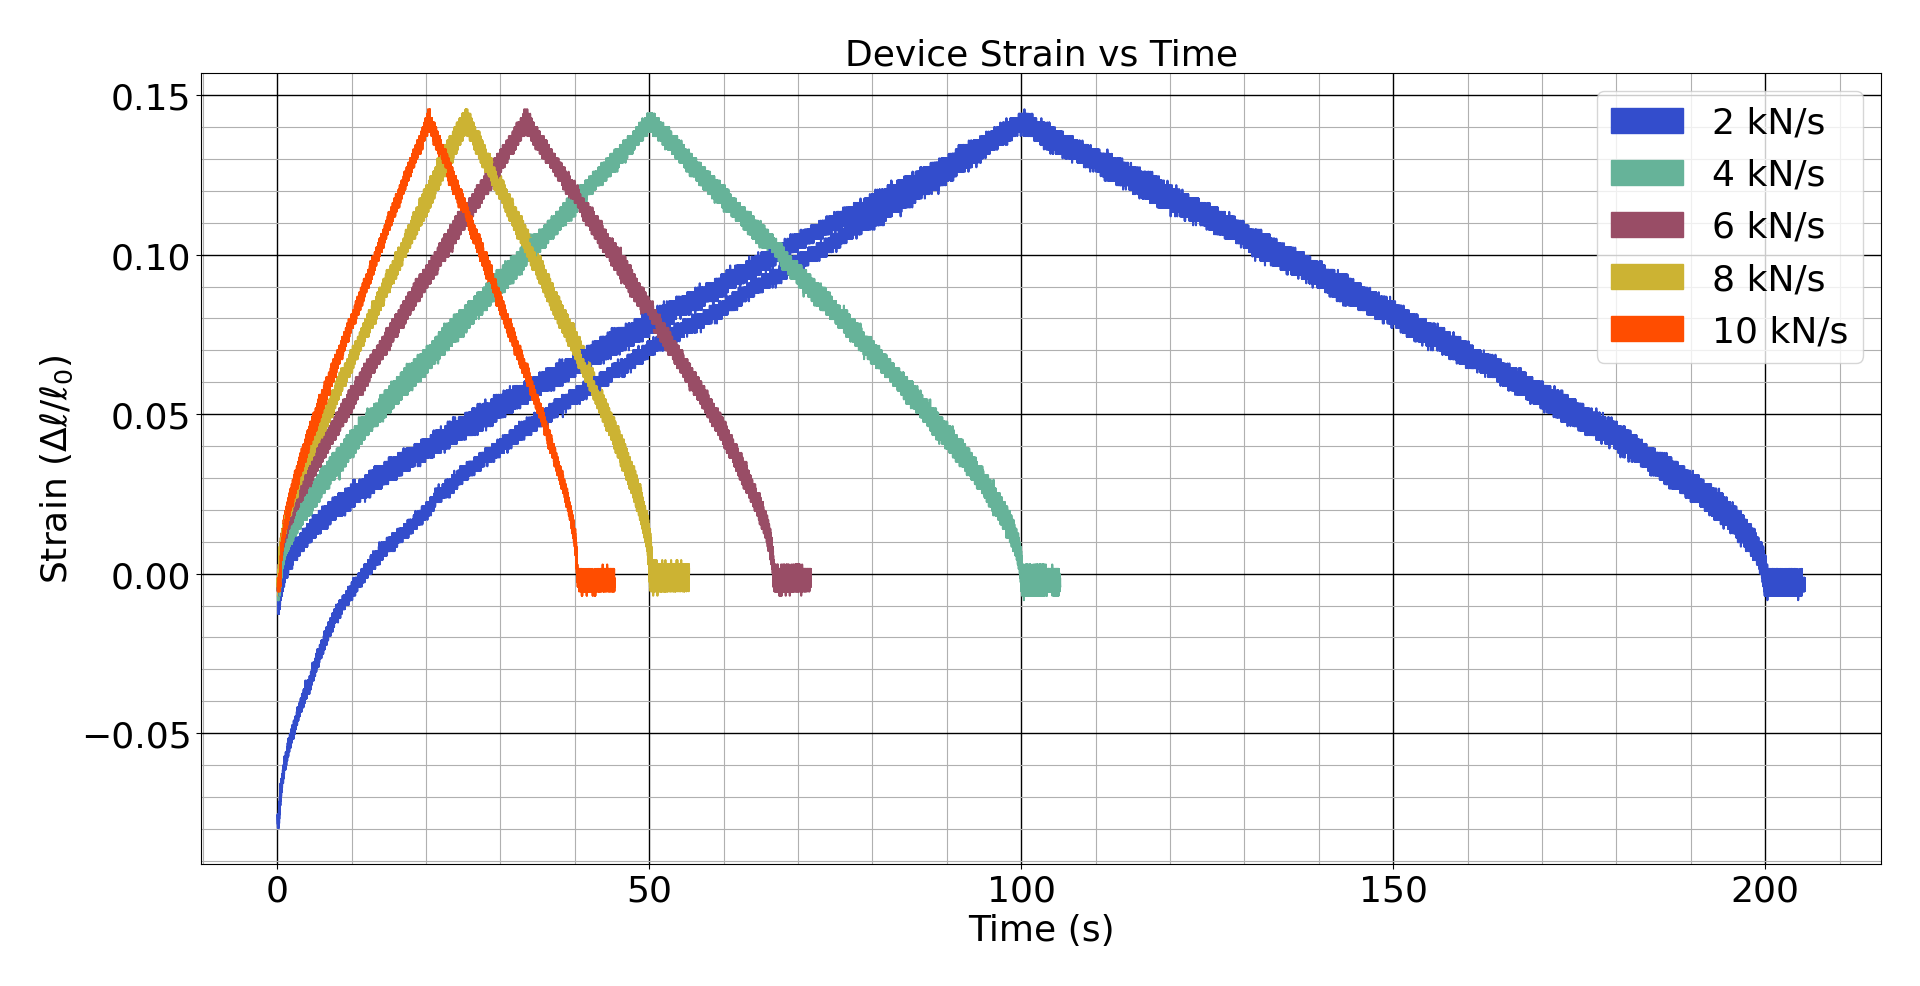
\includegraphics[width=5.5in]{p3_media/figures/combined_strain.png}
\caption{The strain of the physical sensor during the tests. 
This plot shows significant deformation of one of the test sensors during its first loading cycle.
After this first loading cycle, the device strain for each test sensor is similar.
The peak force of each test is 200 kN, and the sensor 
consistently deforms with a strain of 0.14 at this peak.
Considering a sensor height of 1.83 mm, the stiffness, $K_w$, is roughly 780 MN/m.
}
\label{fig:sensor_load_frame_strain}
\end{figure}

\begin{figure}[h]
\centering
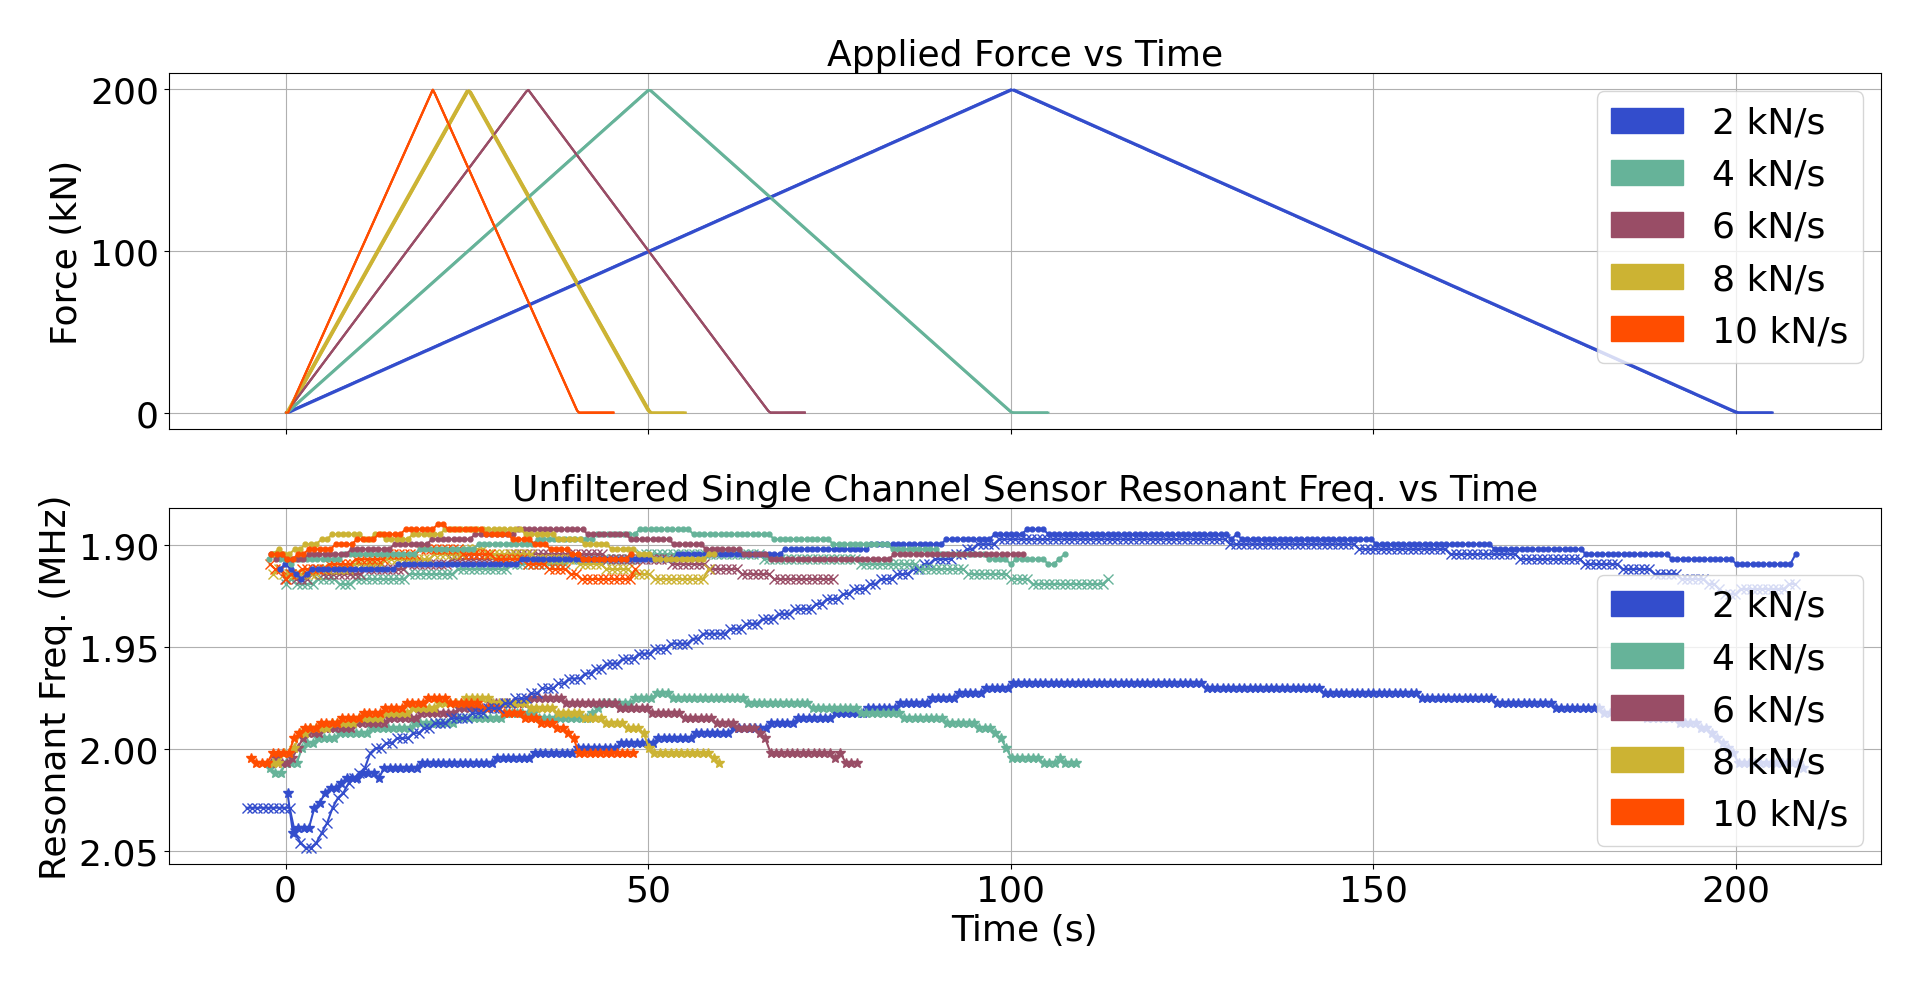
\includegraphics[width=5.5in]{p3_media/figures/combined_load_meas.png}
\caption{Force profiles and cap measurements during loading for the two test sensors. 
The test suite is repeated for the samples not used in the rock test and it gave consistent measurements.
There is some plastic deformation of the steel case during the initial loading of the sensor
in the 2 kN/s case. After this, the sensor has a mostly symmetric response to loading and unloading.
The two sensors have similar sensitivity, but different offsets after the plastic deformation phase.}
\label{fig:sensor_load_frame}
\end{figure}

\FloatBarrier

\begin{figure}[t]
\centering
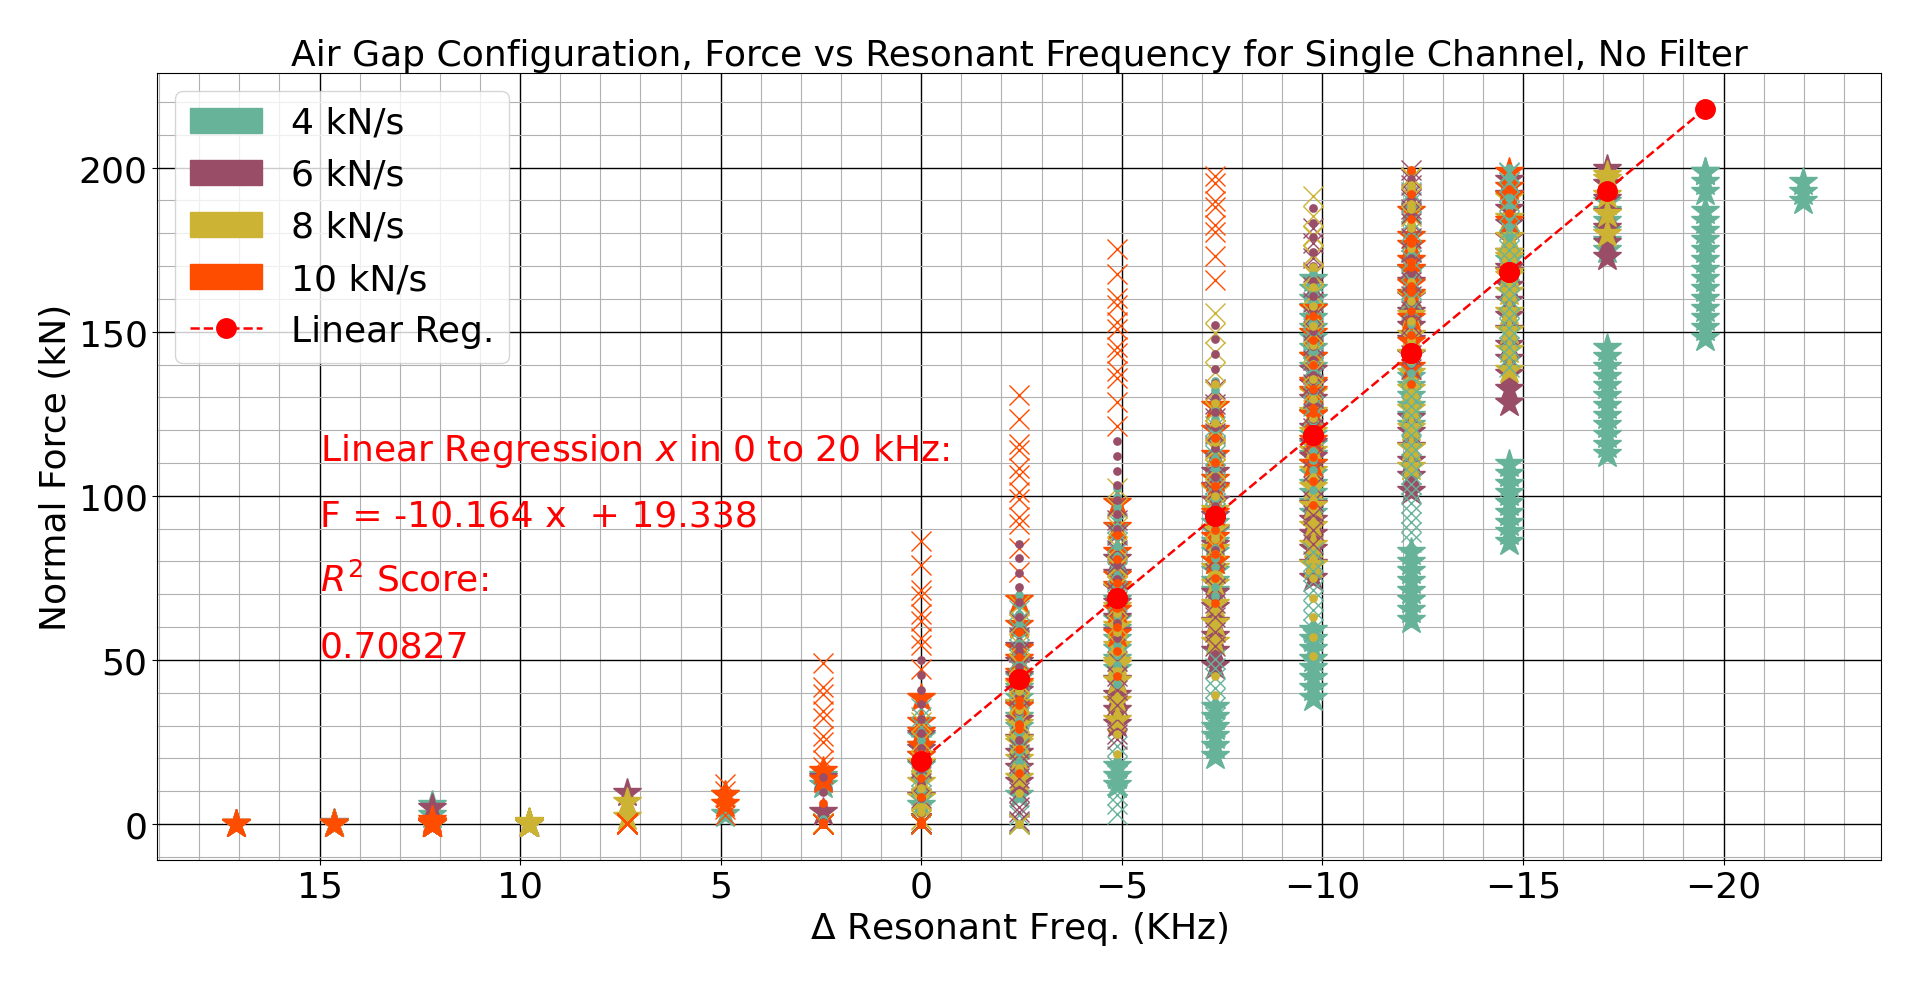
\includegraphics[width=5.5in]{p3_media/figures/combined_force_cap.png}
\caption{The relationship between measured resonant frequency and applied force for each sensor.
The 2 kN/s tests are not representative due to their large, one-time swing in values.
There is some measurement creep, but ramping the input force to 200 kN
will increase the digital sensor measurement roughly 5 to 8 levels. 
The bias for the resonant frequency is reset at the beginning of each test just before
force is applied. 
Compared to the first sensors 4 kN/s test and the second sensors first 10 kN/s test,
most of the other tests have similar measurements.
}
\label{fig:sensor_load_frame_sensitivity}
\end{figure}


\subsubsection{Rock Cutting and Model Fitting}

The initial sensor design was for the air gap configuration. The sensitivity as measured by the 
load frame test was deemed sufficient for binary classification of hard or soft rock.
The fact that the sensor compressed into a more sensitive version under the rock cutting forces
demonstrates that a sensor must be robust to the large forces in this application.
The toughness of the steel and polyimide, and their increased stiffness after compression,
resulted in a usable sensor.

For the rock cutting experiments, we fit the linear model and the other
 empirical models previously discussed in Section~\ref{sub:reg}.
The large number of parameters in the physical model make these regression
techniques a good fit for estimating the cutting force.
Prediction results for a few samples with new picks are shown in \ref{fig:sensor_rock_cut}.
More prediction results using the worn tool are shown in \ref{fig:sensor_rock_cut_worn}.

Using a low pass filter on the sensor measurements improves performance. 
The mean absolute error for each classification method using the different low pass filters is shown in 
\ref{fig:MAE}. The $R^2$ scores are shown in \ref{fig:adjr2}
Using a cutoff frequency of 10 Hz or 5 Hz gave the best results across methods.
The neural network regression method with the 2nd order polynomial expansion performed the best overall.

\FloatBarrier

\begin{figure}[t]
\centering
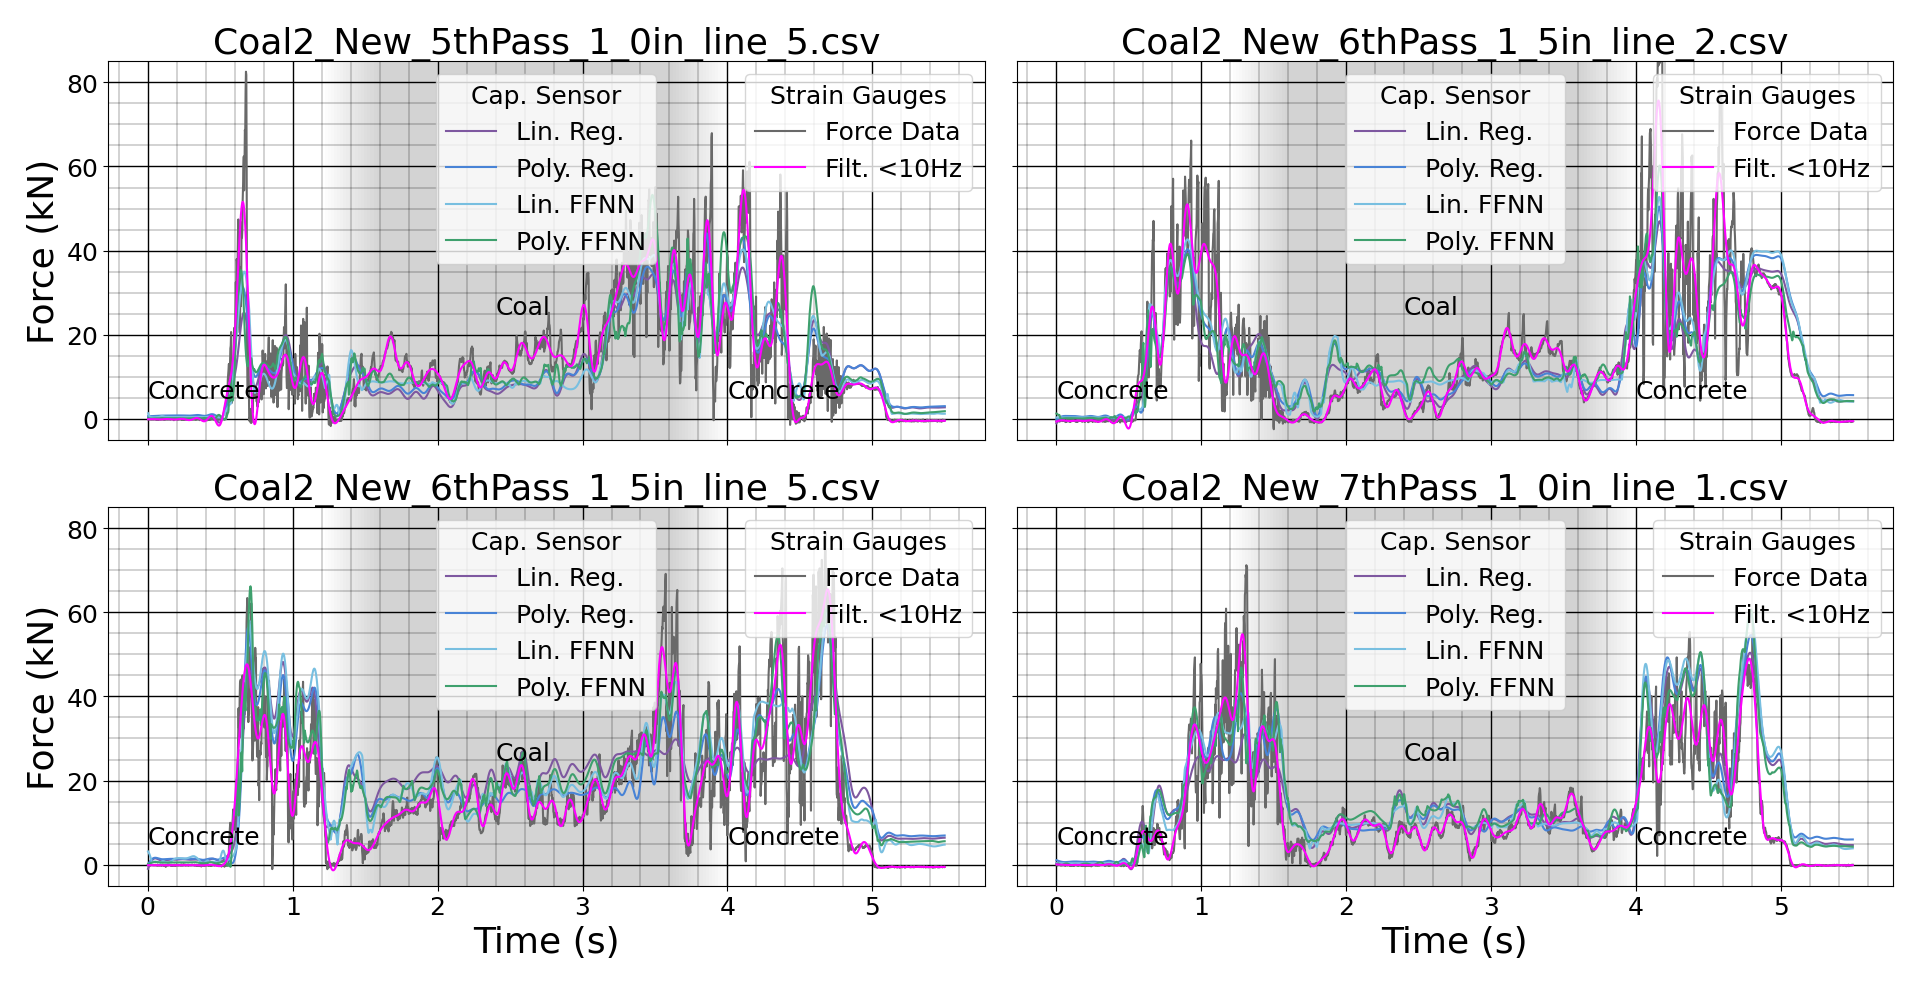
\includegraphics[width=5.0in]{p3_media/figures/model_time_perf.png}
\caption{
Measurements from both the system strain gauges and the custom sensor for the new tool. 
The strain gauge measurements have large variance due to the rock chipping at high frequency.
The regression target is highlighted in magenta. The different regression methods track the force
as the tool cuts through the sample. The middle of the sample is coal, and generally takes less force
to cut than the surrounding concrete.
Our sensor could be used to identify changes in material based on differences in cutting force.
}
\label{fig:sensor_rock_cut}
\end{figure}

\begin{figure}[h]
\centering
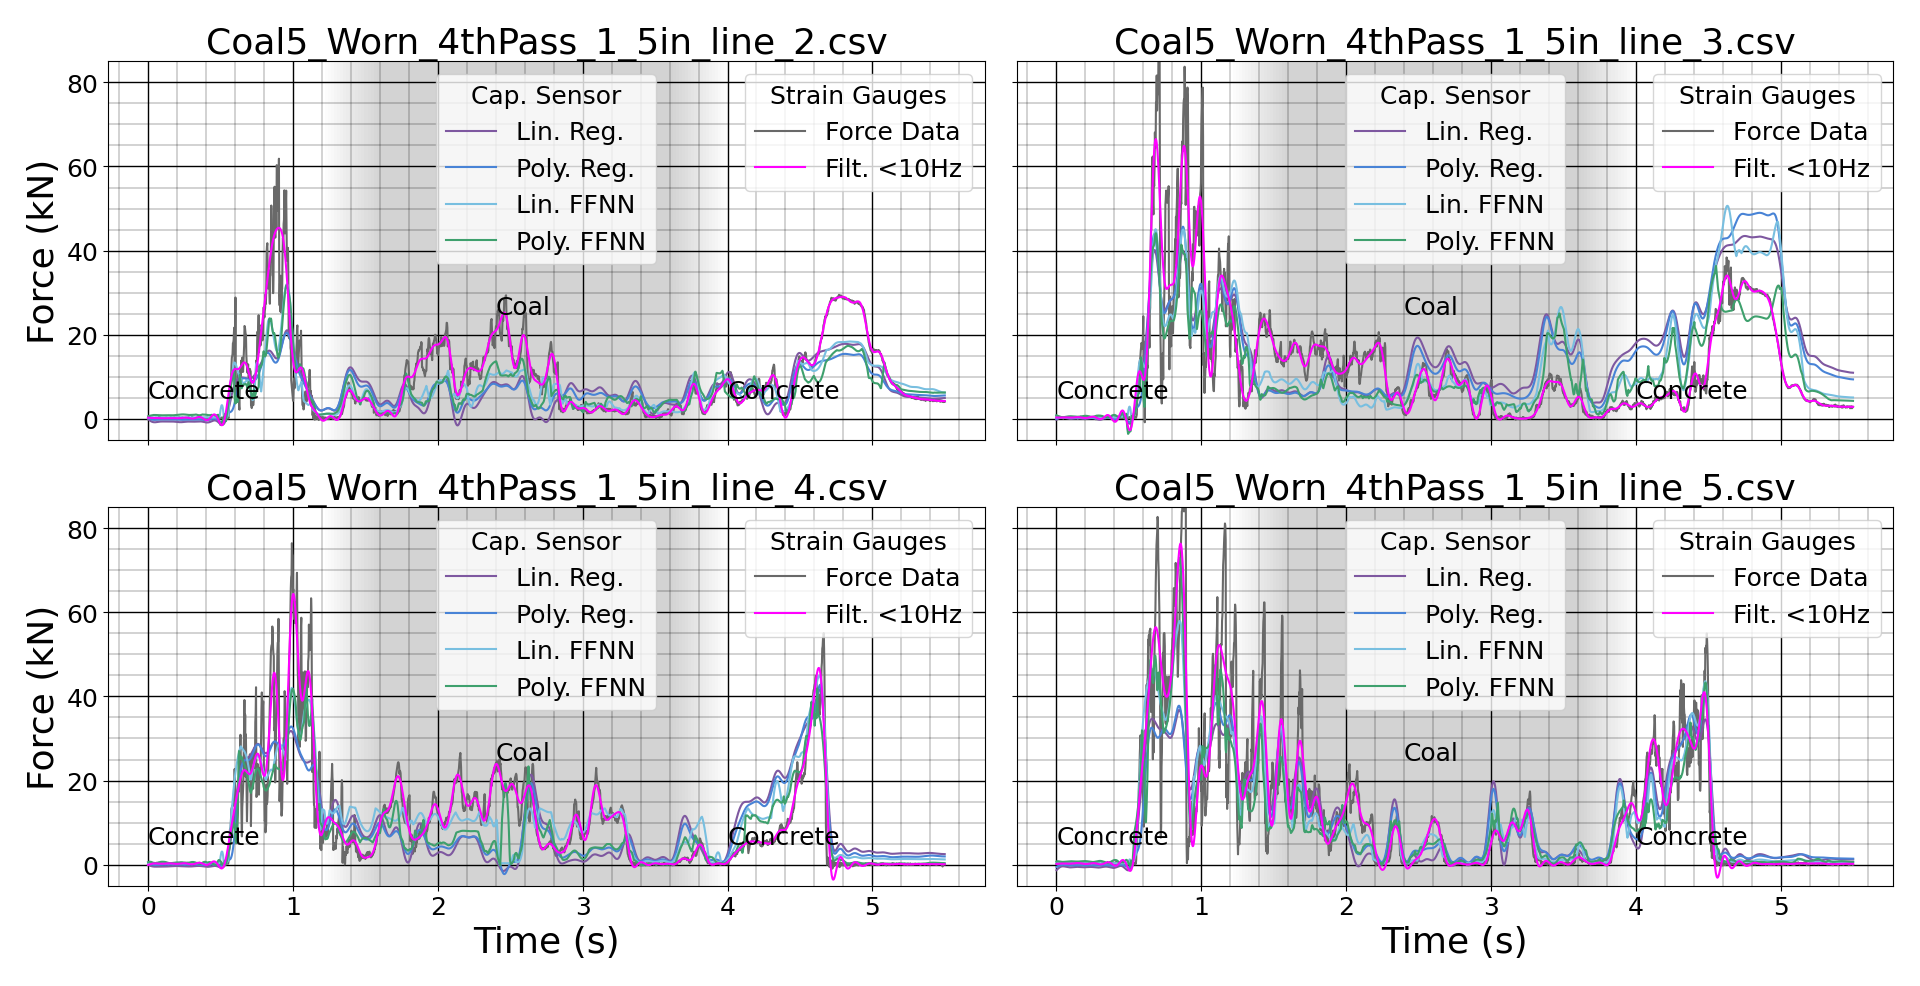
\includegraphics[width=5.0in]{p3_media/figures/model_time_perf_worn.png}
\caption{
Measurements from both the system strain gauges and the custom sensor for the worn tool. 
Use of the worn tool causes greater peak force values in our experiment.
The regression target is highlighted in magenta.
The sensor is able to track the force with the changing wear condition
using the different regression techniques.
Our sensor could be used to detect changes in tool wear based on increases in cutting force
when cutting the same material.
}
\label{fig:sensor_rock_cut_worn}
\end{figure}


\begin{figure}[t]
\centering
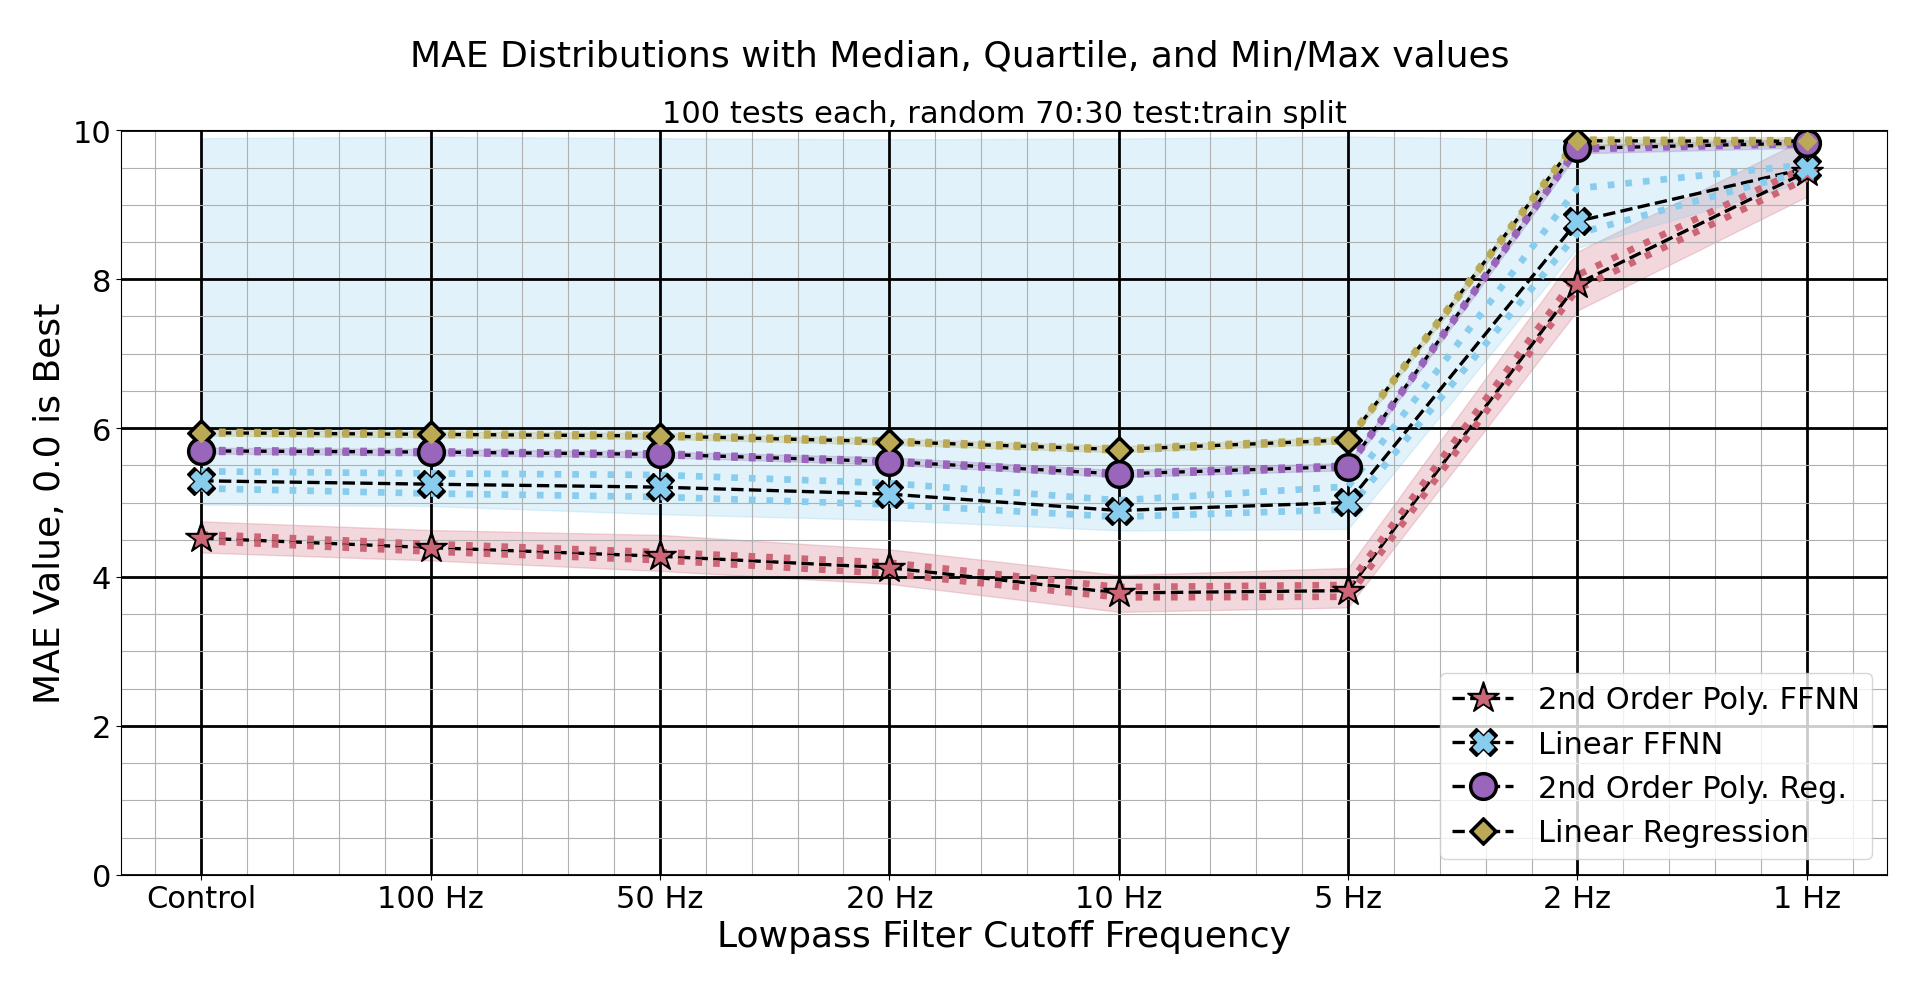
\includegraphics[width=5.0in]{p3_media/figures/mae_perf.png}
\caption{
Mean Absolute Error distributions for different input filter conditions.
The markers and dashed lines represent the median, while the dots and shaded area represent
the quartile and min/max values respectively.
By filtering the measurements
before fitting the regression, we reduce the tracking error.
The performance of the 2nd Order Polynomial Feed-Forward Neural Network
regression breaks away from the rest due to its greater capacity for nonlinear modeling.
}
\label{fig:MAE}
\end{figure}

\begin{figure}[h]
\centering
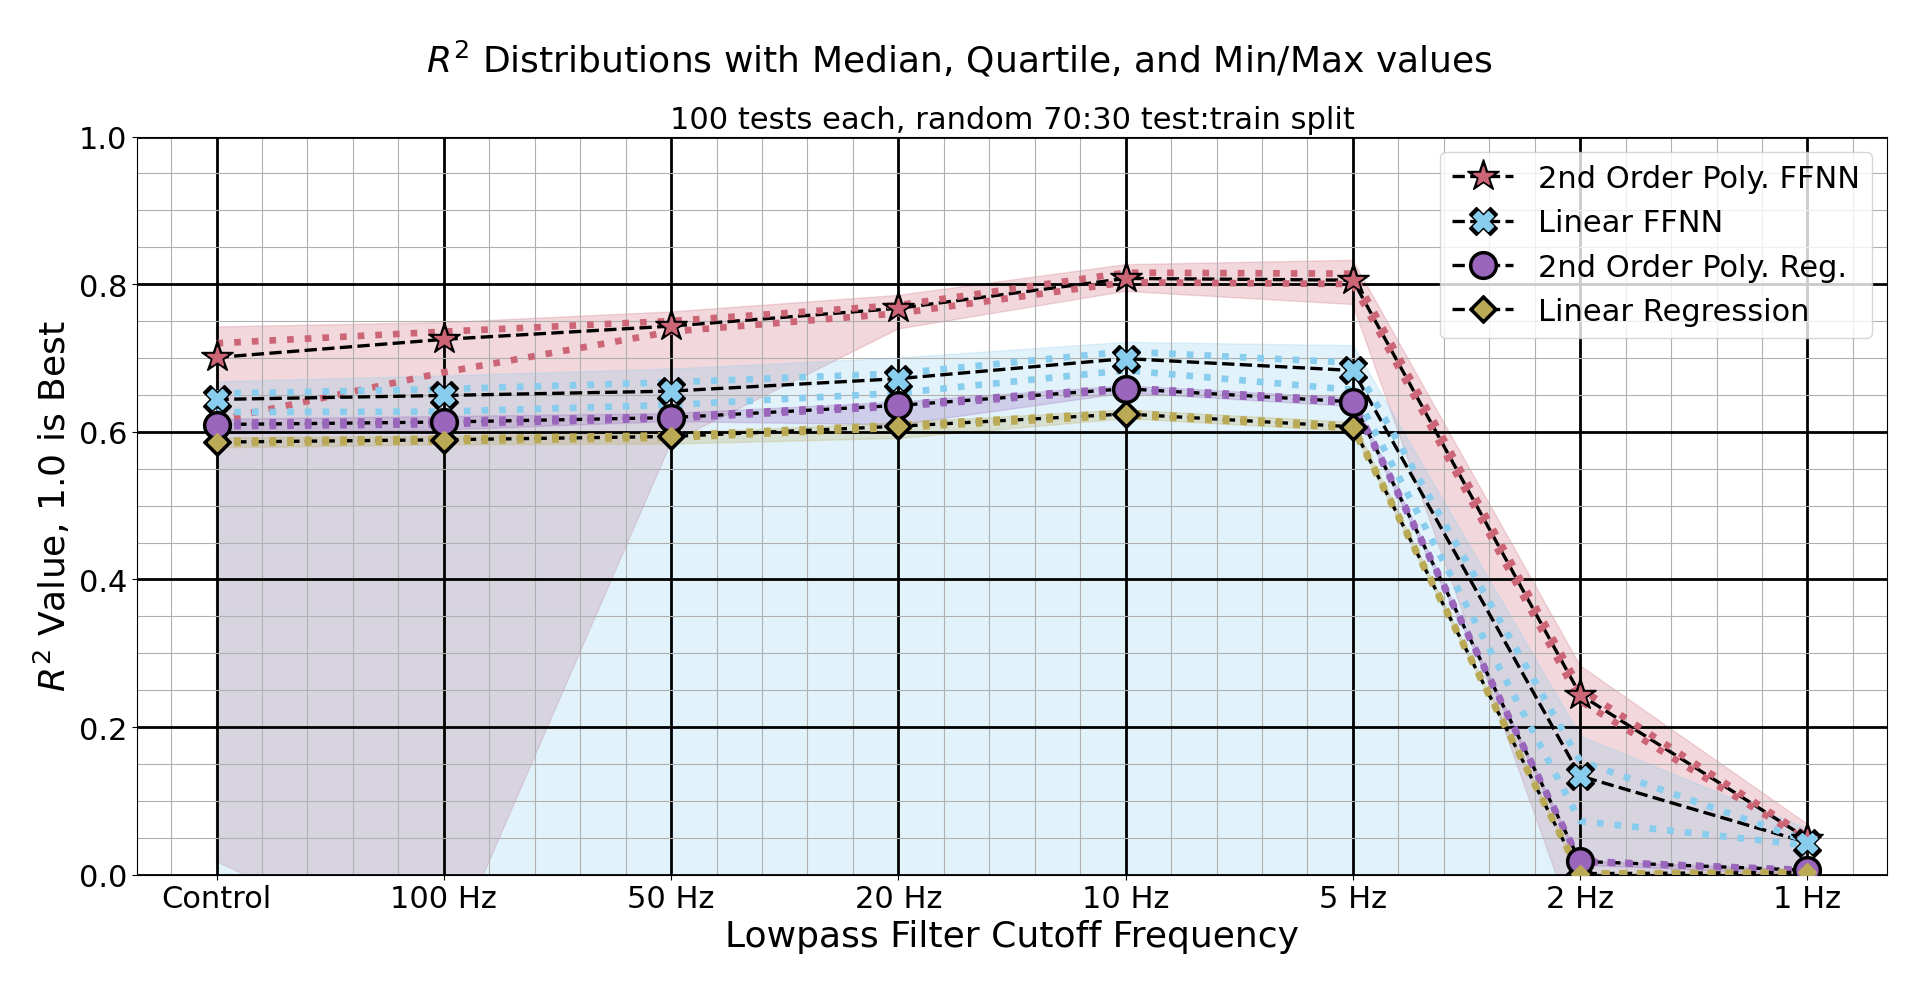
\includegraphics[width=5.0in]{p3_media/figures/r2_perf.png}
\caption{
$R^2$ score distributions for different input filter conditions.
The markers and dashed lines represent the median, while the dots and shaded area represent
the quartile and min/max values respectively.
Using a cutoff frequency the same or slightly lower than the regression target gave 
the best results.
The filtering was needed to make the best performing method reliable, as the control case
gave some regression methods which did not function well.
The regressions without neural networks gave very consistent performance.
} 
\label{fig:adjr2}
\end{figure}

Our analytical models show that the relationship between resonant frequency and input force
is nonlinear, using hyperbolic and inverse square root terms.
Use of the 2nd order polynomial expansion improved results for both 
the linear regression and the neural network regression. 
Use of more sophisticated methods like the neural network regression method
significantly improves performance when used with the 2nd order polynomial expansion.
The neural network without the expanded input was less reliable, with some fraction of the 
trained classifiers always giving bad performance.

\FloatBarrier

\subsection{Discussion}

We choose to track the average normal force, 
as this quantity is known to be correlated with both tool wear and material type.
We average the signal using a low pass filter with a cutoff frequency of 10 Hz 
to allow the higher frequency rock chipping forces to be averaged together while
still allowing a quick response for material and wear changes.
When restricting the regression target bandwidth, we reduce the overall 
variance of the signal. The higher frequency components are not needed to track the average.

Our sensor sensitivity could be improved by using thinner dielectric regions, but care must be taken 
to stay within the linear deformation range for the polyimide material.
Polyimide has linear characteristics for small deformations, but is known
to experience hysteresis and temperature dependence \cite{ZHANG2012, CHO19971615, 7365229}.
The deformation characteristics of thin film polyimide sheets after compression
to a fraction of their original height should be investigated and compared to 
uncompressed sheets of the same height.

The air gap configuration was useful for gentle load profiles and could have applications 
outside of underground mining.
In the rock cutting experiment, the polyimide likely deformed to be much thinner than it was initially.
For the crushed gap configuration, the sensitivity increases to infinity as the layers
become thinner. 
The greater forces result in an increase in sensitivity.


%The sensor performed well for force tracking and could be improved by using larger capacitive pads.
%The few levels of quantization did not inhibit the material differentiation, as the target materials
%of coal and limestone are very distinct. 
%When coupled with our proposed network topology, this sensor could be used to instrument
%each cutting tool on the continous miner cutter head to provide a high-fidelity measurement of 
%both tool wear and material characteristics.

\subsection{Conclusion}\label{sec13}

The sensor performed well for estimating the cutting force, even when using the simple linear regression model.
The ability to track cutting force with a sensor can improve operator performance and safety by giving them
objective feedback while they maintain a safe distance. 
Worker efficiency can be increased via addition of 
autonomous process control enabled by sensors on the continuous miner cutter-head picks.
We have validated our sensor under laboratory conditions and believe this technology is ready
for the next stage of integration with the target application.

Our work shows the implementation of a single sensor.
Forming a network of these sensors would allow the full 
cutter-head state to be known without stopping operations
or requiring and operator to get close to the cutting interface.
Capacitive sensors are a promising technology for applications which 
require low power and low cost.
This work has shown design and validation for two different models of capacitive sensor. 
This design should be easily adaptable to other robotic applications.

%\backmatter
\subsubsection{Acknowledgments}
Special thanks to the Earth Mechanics Institute at
Colorado School of Mines for helping run the experiments.

\subsection*{Declarations}

\subsubsection*{Funding}
This work was funded by NIOSH Contract
75D30119C05413, “IMPROVING HEALTH AND SAFETY OF
MINING OPERATIONS THROUGH DEVELOPMENT OF THE
SMART BIT CONCEPT FOR AUTOMATION OF MECHANICAL
ROCK EXCAVATION UNITS AND DUST MITIGATION.”

\subsubsection*{Conflict of interest}
The authors declare that there is no conflict of interest.

\subsubsection*{Availability of data and materials}
The data used for this research is available publicly at: \\
\url{https://github.com/Fworg64/air_gap_coal_sensor_model}

\subsubsection*{Code availability }
The code used for this research is available publicly at: \\
\url{https://github.com/Fworg64/air_gap_coal_sensor_model}

%\bibliography{airgap-bibliography}% common bib file
